\documentclass[runningheads,a4paper]{llncs}

%%% Some recommended packages.
%\usepackage{booktabs}   %% For formal tables:
%                        %% http://ctan.org/pkg/booktabs
%\usepackage{subcaption} %% For complex figures with subfigures/subcaptions
%                        %% http://ctan.org/pkg/subcaption

% Packages usually used by soton
	% Package for input encoding
	\usepackage[utf8]{inputenc}
	
	%\usepackage[T1]{fontenc}
	%\usepackage{lmodern}
	
	% Package for multilingual support, loaded with English support.
	\usepackage[english]{babel}
	
	% Package for fancy quotations
	\usepackage[autostyle]{csquotes}
	
	% Package for URLs
	\usepackage{url}
	
	\usepackage{colourSoton}
	
	% Package for hyper-references
	\usepackage{hyperref}
	\hypersetup{
		colorlinks=true,
		citecolor=red,
		linkcolor=blue,
		urlcolor=cyan,
	}
	
	% Package for graphics
	\usepackage{graphicx}
	\graphicspath{ {img/} }
	
\usepackage[colorinlistoftodos]{todonotes}

% Package for change tracking
	% \usepackage[disabled]{chgtrk}
	\usepackage{chgtrk}
	\newCTcontributor{Colin}
	\newCTcontributor{Son}
	\newCTcontributor{Karla}
	% \newCTcontributor{Michael}
	
	% Package for abbreviation
	\usepackage{abbrev-scxml2020}
	
	% Package for standalone source code
	\usepackage{standalone}
	
	% Package for requirements document
%	\usepackage[compact]{reqdoc}
	
	% Package for TikZ pictures
	\usepackage{tikz}
	\usetikzlibrary{positioning}
	\usetikzlibrary{shapes}
	
	% Custom pgf pictures
%	\usepackage{pgf-picture}
	
	\usepackage{wrapfig}
	
	% Package for listing Event-B code
	\usepackage[colour]{lstEventB}

	\newtheorem{assumption}{Assumption}
% For floating listings
\usepackage{float}
\newfloat{lstfloat}{htbp}{lop}
\floatname{lstfloat}{Listing}
\def\lstfloatautorefname{Listing} % needed for hyperref/auroref
	
	%package for envelope
	\usepackage{bbding}
% end of packages used by soton

\begin{document}

% first the title is needed
% \title{Refinement of Reactive Systems} 
\title{Formal verification and validation of run-to-completion style statecharts using Event-B}

% a short form should be given in case it is too long for the running head
 \titlerunning{Formal v\&v of statecharts} 

% the name(s) of the author(s) follow(s) next
%
% NB: Chinese authors should write their first names(s) in front of
% their surnames. This ensures that the names appear correctly in
% the running heads and the author index.
%
\author{ 
K. Morris \inst{1} 
\and C. Snook \inst{2}%\textsuperscript{https://orcid.org/0000-0002-0210-0983} 
\and T.S. Hoang \inst{2}
\and \\G. Hulette \inst{1}
\and R. Armstrong \inst{1}
\and M. Butler \inst{2} 
}

\authorrunning{Morris, Snook, Hoang et al.}
%% (feature abused for this document to repeat the title also on left hand pages)

%
% the affiliations are given next; don't give your e-mail address
% unless you accept that it will be published
\institute{
	Sandia National Laboratories, 
	Livermore, California, U.S.A.\\
	% \email{\{knmorri,rob,ghulett\}@sandia.gov}
	\and
	ECS, University of Southampton,
	Southampton, United Kingdom\\
	% \email{\{cfs,t.s.hoang,mjb\}@soton.ac.uk}\\
}


%% \maketitle
%% Note: \maketitle command must come after title commands, author
%% commands, abstract environment, Computing Classification System
%% environment and commands, and keywords command.
\maketitle


% !TEX root = ../main.tex
\begin{abstract}
Text of abstract 
\end{abstract}

\section{Introduction}
We formalise the semantics of refinement in SCXML by modelling, in Event-B,
\begin{itemize}
	\item the structure and behaviour of abstract SCXML models,
	\item the structure, behaviour of refined SCXML models and their relationship to abstract models.
	\item We then refine the latter to remove verification artifacts and show that it is no different to the abstract model and hence SCXML refinement can be applied iteratively.
\end{itemize}

Since SCXML consists of a state-chart behaviour superimposed with a 'run to completion' execution semantics, we formalise the refinement of these two parts separately and then compose the two definitions to obtain the complete SCXMl refinement semantics.
% \section{Introduction}
% Text of paper \ldots
%% !TEX root = ../main.tex

\section{Related Work}
\label{sec:relatedWork}

Many incompatible definitions of refinement have been posed by
others~\cite{Syriani_2019,Maraninchi91theargos} and that can lead to confusion.
Though these separate refinements have different goals, all of which may be
attractive to systems designers in different ways,
% preservation of safety proofs is the goal here. 
%While these other forms of refinement cannot be said to conflict with the one presented here, 
they will not always preserve safety properties.  
From the \EventB vernacular it might be better to relabel these other approaches
not as methods of model ``refinement'', but rather methods of model
``elaboration''.  
Preservation of safety properties across refinement requires only a few
restrictions to the original~\cite{Harel} \SCs (e.g.,transitions cannot cross
containment boundaries arbitrarily), but still allows for both parallel and
hierarchical composition. 
With these restrictions composition becomes a refinement, but not all
refinements are compositions.  
Such a unification of composition and refinement can lead, not only to code
reuse, but reuse of proofs.

If an \EventB\ model |B| can be shown (via the construction rules of the \EventB
language as well as the proof obligations) to refine another \EventB
model |A|, then we know that every behavior of |B| is also a behavior
of |A|. This definition yields a useful principle of preservation of
safety -- if we can show that a bad thing never happens in |A|, then
we can add detail via refinements in |B|, knowing that the bad thing
will continue to never happen in |B|. That is, \EventB refinements
preserve safety properties in the sense adopted by Lamport
~\cite{lamport1977proving}. This makes refinement a useful technique
in developing safety-critical systems: one can analyze a simpler
abstract model for critical safety properties and then add detail to
the model via refinements, secure in the knowledge that the safety
properties will be preserved. While \EventB refinements have also been
shown to preserve some liveness properties under certain
conditions~\cite{hoang2016ltl}, there are not yet efficient supporting
tools for the technique. Instead, we can express the property in \LTL
and use the \PROB\footnote{ProB is an animator, constraint solver and
  model checker for the B-Method. \url{https://www3.hhu.de/stups/prob}}
model checker to verify it, as we have shown in previous
work~\cite{detect2020}.  In this paper, we outline a proof of liveness
properties that relies on reasoning about deadlock-freeness and event
convergence.

\SonAdd{%
  A method that is closely related to \mbox{\EventB} and also supports
  reasoning about safety and liveness properties is
  TLA+~\mbox{\cite{DBLP:books/aw/Lamport2002}}. TLA+ is supported by
  the TLA+ Toolbox~\mbox{\cite{DBLP:journals/corr/abs-1912-10633}}.
  On the one hand, temporal properties (both safety and liveness) are
  \emph{explicitly} stated as properties of the TLA+ models and
  reasoning about them often requires applying proof rules related to
  properties of traces. On the other hand, \mbox{\EventB} defines
  proof obligations based on the underlying trace
  semantics~\mbox{\cite{abrial10:_model_event_b,hoang2016ltl,hudon16:_unit_b_method}},
  hence reasoning about \emph{implicitly} temporal properties in
  \mbox{\EventB} simply involves discharging the relevant proof
  obligations. Furthermore, at the time of writing, the TLA+ Proof
  System (part of the TLA+ Toolbox) does not fully support the
  reasoning with many temporal operators.%
}%
\footnote{\url{http://tla.msr-inria.inria.fr/tlaps/content/Documentation/Unsupported_features.html}
  (accessed June 2021)}

%%%%%%%%%%%%%%%%%%%%%%%%%%%%%%%%%%%%%%%%%%%%%%%%%%%%%%%%%%%%%%%%%%%%%%%%



% Previous work has developed a number of different semantics all with different purposes and outcomes~\cite{Syriani_2019,Harel,Maraninchi91theargos}.  
% Because this work is focused on a mapping to \EventB, safety property preserving refinement is key.  
% \EventB provides not only a definition of refinement but a rubric for finding valid refinements and this is carried over into the \SCs work presented here. 
% In our version of \SC semantics, refinement means a subsetting of traces from an abstraction. 
% This has the beneficial effect of preserving safety properties from abstraction to refinement and permits proofs to be
% discharged at the highest tractable level of abstraction.
% It is at the highest level of abstraction that proofs are presumably the easiest to discharge.

% Many incompatible definitions of refinement have been posed by others~\cite{Syriani_2019,Maraninchi91theargos} and that can lead to confusion.  
% Though these separate refinements have different goals, all of which may be attractive to systems designers in different ways, preservation of safety proofs is the goal here. 
% While these other forms of refinement cannot be said to conflict with the one presented here, they will not always preserve safety properties.  
% From the \EventB vernacular it might be better to relabel these other approaches not as methods of model ``refinement'', but rather methods
% of model ``elaboration''.  


% Preservation of safety across refinement requires only a few restrictions to the original~\cite{Harel} \SCs (e.g. transitions cannot
% cross containment boundaries arbitrarily), but still allows for both parallel and hierarchical composition. 
% With these restrictions composition becomes a refinement, but not all refinements are compositions.  
% Such a unification of composition and refinement can lead, not only to code reuse, but reuse of proofs.

%%%%%%%%%%%%%%%%%%%%%%%%%%%%%%%%%%%%%%%%%%%%%%%%%%%%%%%%%%%%%%%%%%%%%%%%




% Although the autonomous drone example in this paper is based on the
% example described in~\cite{Syriani_2019}, the definition of refinement
% used in that work is quite different from our own. This forces some
% differences in our refinement rules and consequently the way the
% example is developed.  In~\cite{Syriani_2019} ``refinement'' is a
% transformation of the model which preserves reachability of a state
% with respect to sequences of inputs. However, this also allows the
% possibility of introducing new behaviors in the concrete model that
% the abstraction does not exhibit (more details are in
% Section~\ref{sec:descr-sample-appl}). While this notion of refinement
% seems useful in certain contexts, unlike refinement in \EventB it does
% not guarantee preservation of safety properties. Therefore it should
% be considered less suited to development of safety-critical systems.

%%% Local Variables:
%%% mode: latex
%%% TeX-master: "../main"
%%% End:
% !TEX root = ../main.tex

\section{Background}
\label{sec:background}
 
% !TEX root = ../main.tex

\subsection{Event-B}
\label{sec:eventb}

\EventB~\cite{abrial10:_model_event_b,hoang13:_introd_event_b_model_method} is a formal method for system
design.  It uses \emph{refinement} to introduce system details gradually into the
formal model.  An \EventB model contains two parts: \emph{contexts} and \emph{machines}. 
Contexts contain \emph{carrier sets}, \emph{constants}, and \emph{axioms} constraining 
the carrier sets and constants.  Machines contain \emph{variables} |v|, \emph{invariants} |I(v)| 
constraining the variables, and \emph{events}. An event consists of a guard 
denoting its enabled-condition and an action defining the value of variables after the event is executed.  
In general, an event |e| has the form: |any t where G(t, v) then S(t, v) end| where |t| 
are the event parameters, |G(t, v)| is the guard of the event, and |S(t, v)| is the action of the event.
% \begin{center}
  % |any t where G(t, v) then S(t, v) end|
%& \inlineevent{\Be}{}{\Bt}{G(\Bt,\Bv)}{}{S(\Bt,\Bv)}
% \end{center}
%In the case where the event has no parameters, we use the following form
%\begin{center}
%  |when G(v) then S(v) end|
%%& \inlineevent{\Be}{}{}{G(\Bv)}{}{S(\Bv)}~,
%\end{center}
% and when the event has no parameters and no guard, we use
% \begin{center}
%   |begin S(v) end|
% %& \inlineevent{\Be}{}{}{}{}{S(\Bv)}~.
% \end{center}
%The action of an event comprises of one or more assignments, each of them has one of the following forms: (1) |v := E(t, v)|, (2) |v :: E(t, v)|, and (3) |v :∣ P(t, v)|.  Assignments of form (1) are deterministic, assign the value of expression |E(t, v)| to |v|.  Assignments of forms (2) and (3) are non-deterministic. (2) assigns any value from the set |E(t,v)| to |v|, while (3) assigns any value satisfied predicate |P(t,v)| to |v|.
%A machine in \EventB corresponds to a transition system
%where \emph{variables} represent the states and \emph{events} specify
%the transitions.  Note that invariants |I(v)| are inductive, i.e., they must be \emph{maintained} by all events. This is more strict than general safety properties which hold for all reachable states of the \EventB machine.  
% This is also the difference between verifying the consistency of \EventB machines using theorem proving and model checking (e.g., \PROB) techniques: model checkers explore all reachable states of the system while interpreting the invariants as safety properties.  

Machines can be refined by adding more details.  Refinement can be done by extending the machine 
to include additional variables (\emph{superposition refinement}) representing new features of 
the system, or by replacing some (abstract) variables by new (concrete) variables (\emph{data refinement}).  
% More information about \EventB can be found
% in~\cite{hoang13:_introd_event_b_model_method}.
Refinement in \EventB is reasoned on an event basis.  
A (concrete) event |f| refines an (abstract) event |e| if whenever |f| is enabled then |e| is also enabled (guard strengthening), and the action of |f| is the same or equivalent to |e| (where equivalence is given by some relationship defined in the invariants). 
New events are said to refine `skip' (an implicit abstract event that did nothing), and therefore do not alter abstract variables.
 More information about \EventB refinement can be
found in~\cite{abrial10:_model_event_b}.
\EventB is supported by the Rodin Platform (Rodin\footnote{An extensible toolkit which includes 
facilities for modelling, verifying the consistency of models using theorem proving and model 
checking techniques, and validating models with simulation-based approaches.})~\cite{abrial10:_rodin}.

\hl{Proof obligations are generated to ensure the consistency of
  \mbox{\EventB} models.  An important proof obligation in
  \mbox{\EventB} is invariant preservation to prove that safety
  properties (encoded as invariants of the models) will not be
  violated for any reachable states.  In this paper, we also make use
  of other proof obligations in \mbox{\EventB} such as (relative)
  deadlock-freeness and (conditional) event convergence to construct
  our proof of liveness properties under some fairness
  assumptions.%
}

\hl{%
  For the trace semantics corresponding to \mbox{\EventB} machines and
  the interpretation of LTL properties over traces, we refer the readers
  to \mbox{\cite{hoang2016ltl}}.  Here, we recall the notation for
  fairness assumptions underlying event-based formalisms such as
  \mbox{\EventB~\cite{lamport1977proving,hudon16:_unit_b_method}}. Given
  an event \mbox{\EventBInline{e}}, a weak-fairness assumption
  \mbox{\EventBInline{WF(e)}} states that if \mbox{\EventBInline{e}}
  is enabled continually, then it must occur infinitely often.
  Similarly, a strong-fairness assumption \mbox{\EventBInline{SF(e)}}
  states that if \mbox{\EventBInline{e}} is enabled infinitely often,
  then it must occur infinitely often. Formally,
}
\begin{center}
  \EventBInline{WF(a)  <=> (FG enabled(e) => GF [e])}, and

  \EventBInline{SF(a)  <=> (GF enabled(e) => GF [e])},
\end{center}
\hl{%
  where \mbox{\EventBInline{G}} and \mbox{\EventBInline{F}} are the
  temporal operators denoting \emph{globally}, and \emph{finally},
  respectively; and \mbox{\EventBInline{enabled(e)}} denotes that
  event \mbox{\EventBInline{e}} is enabled and
  \mbox{\EventBInline{[e]}} denotes an occurrence of event
  \mbox{\EventBInline{e}}.
}
% In \EventB the run to completion pseudocode of Listing~\ref{lst:scxml-r2c} could be represented (somewhat abstractly) as shown in Listing~\ref{lst:eventb-r2c}.
% \begin{lstlisting}[caption={Run to completion pseudocode in \EventB},label={lst:eventb-r2c}, language=Event-B, escapechar=|, frame=single, float=t]
%  FireUntriggered // Fire  enabled un-triggered transitions
% when
%     UC = FALSE // Has not yet completed firing un-triggered transitions
%     untriggered() /= {}
% then
%     execute(untriggered()) // Execute enabled un-triggered transitions
% end
% UntriggeredCompleted // Un-triggered transitions are completed
% when
%     UC = FALSE // Has not yet completed firing un-triggered transitions
%     untriggered() = {} // No more enabled un-triggered transitions
% then
%     UC = TRUE // Complete firing un-triggered transitions
% end
% FireInternallyTriggered // Fire an internal trigger
% when
%     UC = TRUE // Complete firing un-triggered transitions
%     IQ /= {} // The internal triggers queue is non-empty
% then
%     execute(IQ.dequeue) // Execute and dequeue from the internal triggers queue
%     UC := FALSE // Re-enable firing of un-triggered transitions
% end
% FireExternallyTriggered // Fire an external trigger
% when
%     UC = TRUE // Complete firing un-triggered transitions
%     IQ = {} // The internal trigger queue is empty
%     EQ /= {} // The external trigger queue is non-empty
% then
%     execute(EQ.dequeue)  // Execute and dequeue from the external triggers queue
%     UC := FALSE // Re-enable firing of un-triggered transitions
% end
% \end{lstlisting}	
% Here, |IQ| and |EQ| are queues of internally and externally, raised triggers, |untriggered| selects a set of currently enabled un-triggered transitions, |dequeue| retrieves the next trigger from the given queue and selects the set of transitions that become enabled by it and |execute| fires the given set of transitions. 
% Note that this is an abstract representation where each event (|FireUntriggered|, |FireInternallyTriggered|, and |FireExternallyTriggered|) would be specialised to select a particular set of transitions that can be fired in parallel and |execute()| would be replaced by actions that encode the state changes made by those transitions.
% Representing the condition \textbf{untriggered\_enabled} (Line 3 in Listing~\ref{lst:scxml-r2c}) is cumbersome since we would need to write a conjunction of all the possible un-triggered guards. Instead we introduce a dummy un-triggered event that is only fired when no other selection of un-triggered transitions are available and sets a boolean flag, |UC|, to indicate that none of the real un-triggered events was fired and a trigger needs to be consumed.
 
% Note that causing all of the
% transitions to simultaneously and atomically fire for each event is a
% further semantic choice.  Transitions associated with |FireUntriggered|,
% |FireInternallyTriggered|, and |FireExternallyTriggered| might
% just as well fire separately in a non-deterministic order, or by use
% of a per-transition priority, fire in a predetermined order.  Each
% choice has realistic exemplars in the physical world, and to some
% degree, the choice is arbitrary.  The argument in favour of the
% parallel atomic transitions chosen here is pragmatic: the resulting
% representation in \EventB is more terse.

%%% Local Variables:
%%% mode: latex
%%% TeX-master: "../main"
%%% End:

% !TEX root = ../main.tex

\subsection{UML-B State-machines}
\label{sec:iumlb}

\UMLB~\cite{said15:umlbSosym,snook14:iumlbStatem,snook06umlbTosem} provides a diagrammatic modelling notation for \EventB in the form of state-machines and class diagrams. 
The diagrammatic models relate to an \EventB machine and generate or contribute to parts of it. 
For example a state-machine will automatically generate the \EventB data elements (sets, constants, axioms, variables, and invariants) to implement the states. 
Transitions contribute further guards and actions representing their state change, to the events that they elaborate.  
State-machines are typically refined by adding nested state-machines to states.
% Figure~\ref{fig:iumlb-sm} shows an example of a simple state-machine with two states.
% \begin{figure}[!h]
% 	\vspace{-.5cm}
% 	\centering
% 	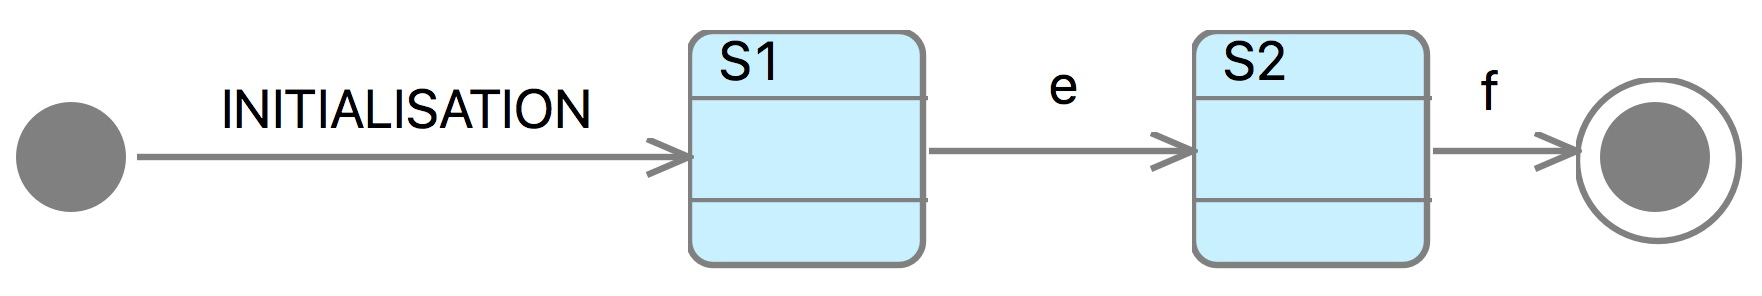
\includegraphics[width=0.6\textwidth]{figures/iumlb-SM}
% 	\caption{An example \UMLB state-machine}
% 	\label{fig:iumlb-sm}
% 	\vspace{-.5cm}
% \end{figure}

Each state is encoded as a boolean variable and the current state is indicated by one of the boolean variables being set to |TRUE|. 
An invariant ensures that only one state is set to |TRUE| at a time.
%The state-machine, is initialised by setting one state variable to |TRUE| and all others to |FALSE|.
Events change the values of state variables to move the |TRUE| value according to the transitions in the state-machine.  
% The \EventB translation%
% %
% \footnote{%
%   Here, $\mathrm{partition(S, T1, T2, \ldots)}$ means the set $S$ is partitioned into disjoint (sub-)sets $T1, T2, \ldots$.
% that cover $S$} 
% of the state-machine in Figure~\ref{fig:iumlb-sm} can be seen in Listing~\ref{lst:eventb-sm}.
% \UMLB also provides the option of an alternative translation with a single state variable ranging over an enumerated type of states, however, the boolean representation of each state is more natural for a user to reference in \SCXML guards and actions.
	
While the \UMLB translation deals with the basic data formalisation of state-machines it differs 
significantly from the semantics discussed in this manuscript. 
\UMLB adopts \EventB's simple guarded action semantics and does not have a concept of triggers and run-to-completion.
Here we make use of \UMLB's state-machine translation but provide a completely different semantic by generating a behaviour into the underlying \EventB events that are linked to the generated \UMLB transitions.
% \begin{lstlisting}[caption={Translation of the state-machine in Fig.~\ref{fig:iumlb-sm}},label={lst:eventb-sm}, language=Event-B, escapechar=|, frame=single]
% variables S1 S2
% invariants 
% 	TRUE !: {S1, S2} => partition({TRUE}, {S1}/\{TRUE}, {S2}/\{TRUE})
% events
%     INITIALISATION: begin S1, S2 := TRUE, FALSE end
%     e: when S1 = TRUE then S1, S2 ≔ FALSE, TRUE  end
%     f: when S2 = TRUE then S2 := FALSE end
% end
% \end{lstlisting}
%%% Local Variables:
%%% mode: latex
%%% TeX-master: "../main"
%%% End:

% !TEX root = ../main.tex

\subsection{SCXML}
\label{sec:scxml}

\SCXML is a modelling language based on Harel statecharts with facilities for adding data elements that are manipulated by transition actions and used in conditions for their firing. \SCXML follows the usual `run to completion' semantics of such statechart languages, where trigger events\footnote{In \SCXML the triggers are called `events', however, we refer to them as `triggers' to avoid confusion with \EventB} may be needed to enable transitions. Trigger events are queued when they are raised, and then one is de-queued and consumed by firing all the transitions that it enables, followed by any (un-triggered) transitions that then become enabled due to the change of state caused by the initial transition firing. This is repeated until no transitions are enabled, and then the next trigger is de-queued and consumed. There are two kinds of triggers: internal triggers are raised by transitions and external triggers are raised by the environment (spontaneously as far as our model is concerned). An external trigger may only be consumed when the internal trigger queue has been emptied. 

\begin{lstlisting}[caption=Pseudocode for 'run to completion',label={lst:scxml-r2c}, frame=single]
while running:
	while completion = false
		if untriggered_enabled
			execute(untriggered())
		elseif IQ /= {}
			execute(internal(IQ.dequeue)) 
		else
			completion = true
		endif
	endwhile
	if EQ /= {}
		execute(EQ.dequeue) 
		completion = false
	endif
endwhile 
\end{lstlisting}

Listing~\ref{lst:scxml-r2c} shows a pseudocode representation of the run to completion semantics as defined within the latest W3C recommendation document~\cite{scxmlwebsite}. Here IQ and EQ are the triggers present in the internal and external queues respectively. We adopt the commonly used terminology where a single transition is called a \emph{micro-step} and a complete run (between de-queueing external triggers) is referred to as a \emph{macro-step}.

%%% Local Variables: 
%%% mode: latex
%%% TeX-master: "../main.tex"
%%% End: 


%%% Local Variables:
%%% mode: latex
%%% TeX-master: "../main"
%%% End:

% !TEX root = ../main.tex


\section{Run To Completion}
\label{sec:run-completion}
The run to completion semantics is specified via an abstract basis that is extended by the model~\cite{MoSnHo18,MoSnHo-ABZ2020}. 
Figure~\ref{fig:basis} shows a state-chart representation of how the basis enforces 
the run to completion semantics on the model transitions. 

\ColinInlineComment{the Fig.1 needs updating wrt to queues.. e.g. eQ and iQ should be content(eQ) and content(iQ).
	also NoTriggeredTransitionsEnable should be NoTriggeredTransitionsEnabled}
\begin{figure}[!h]
	\vspace{-.4cm}
	\centering
	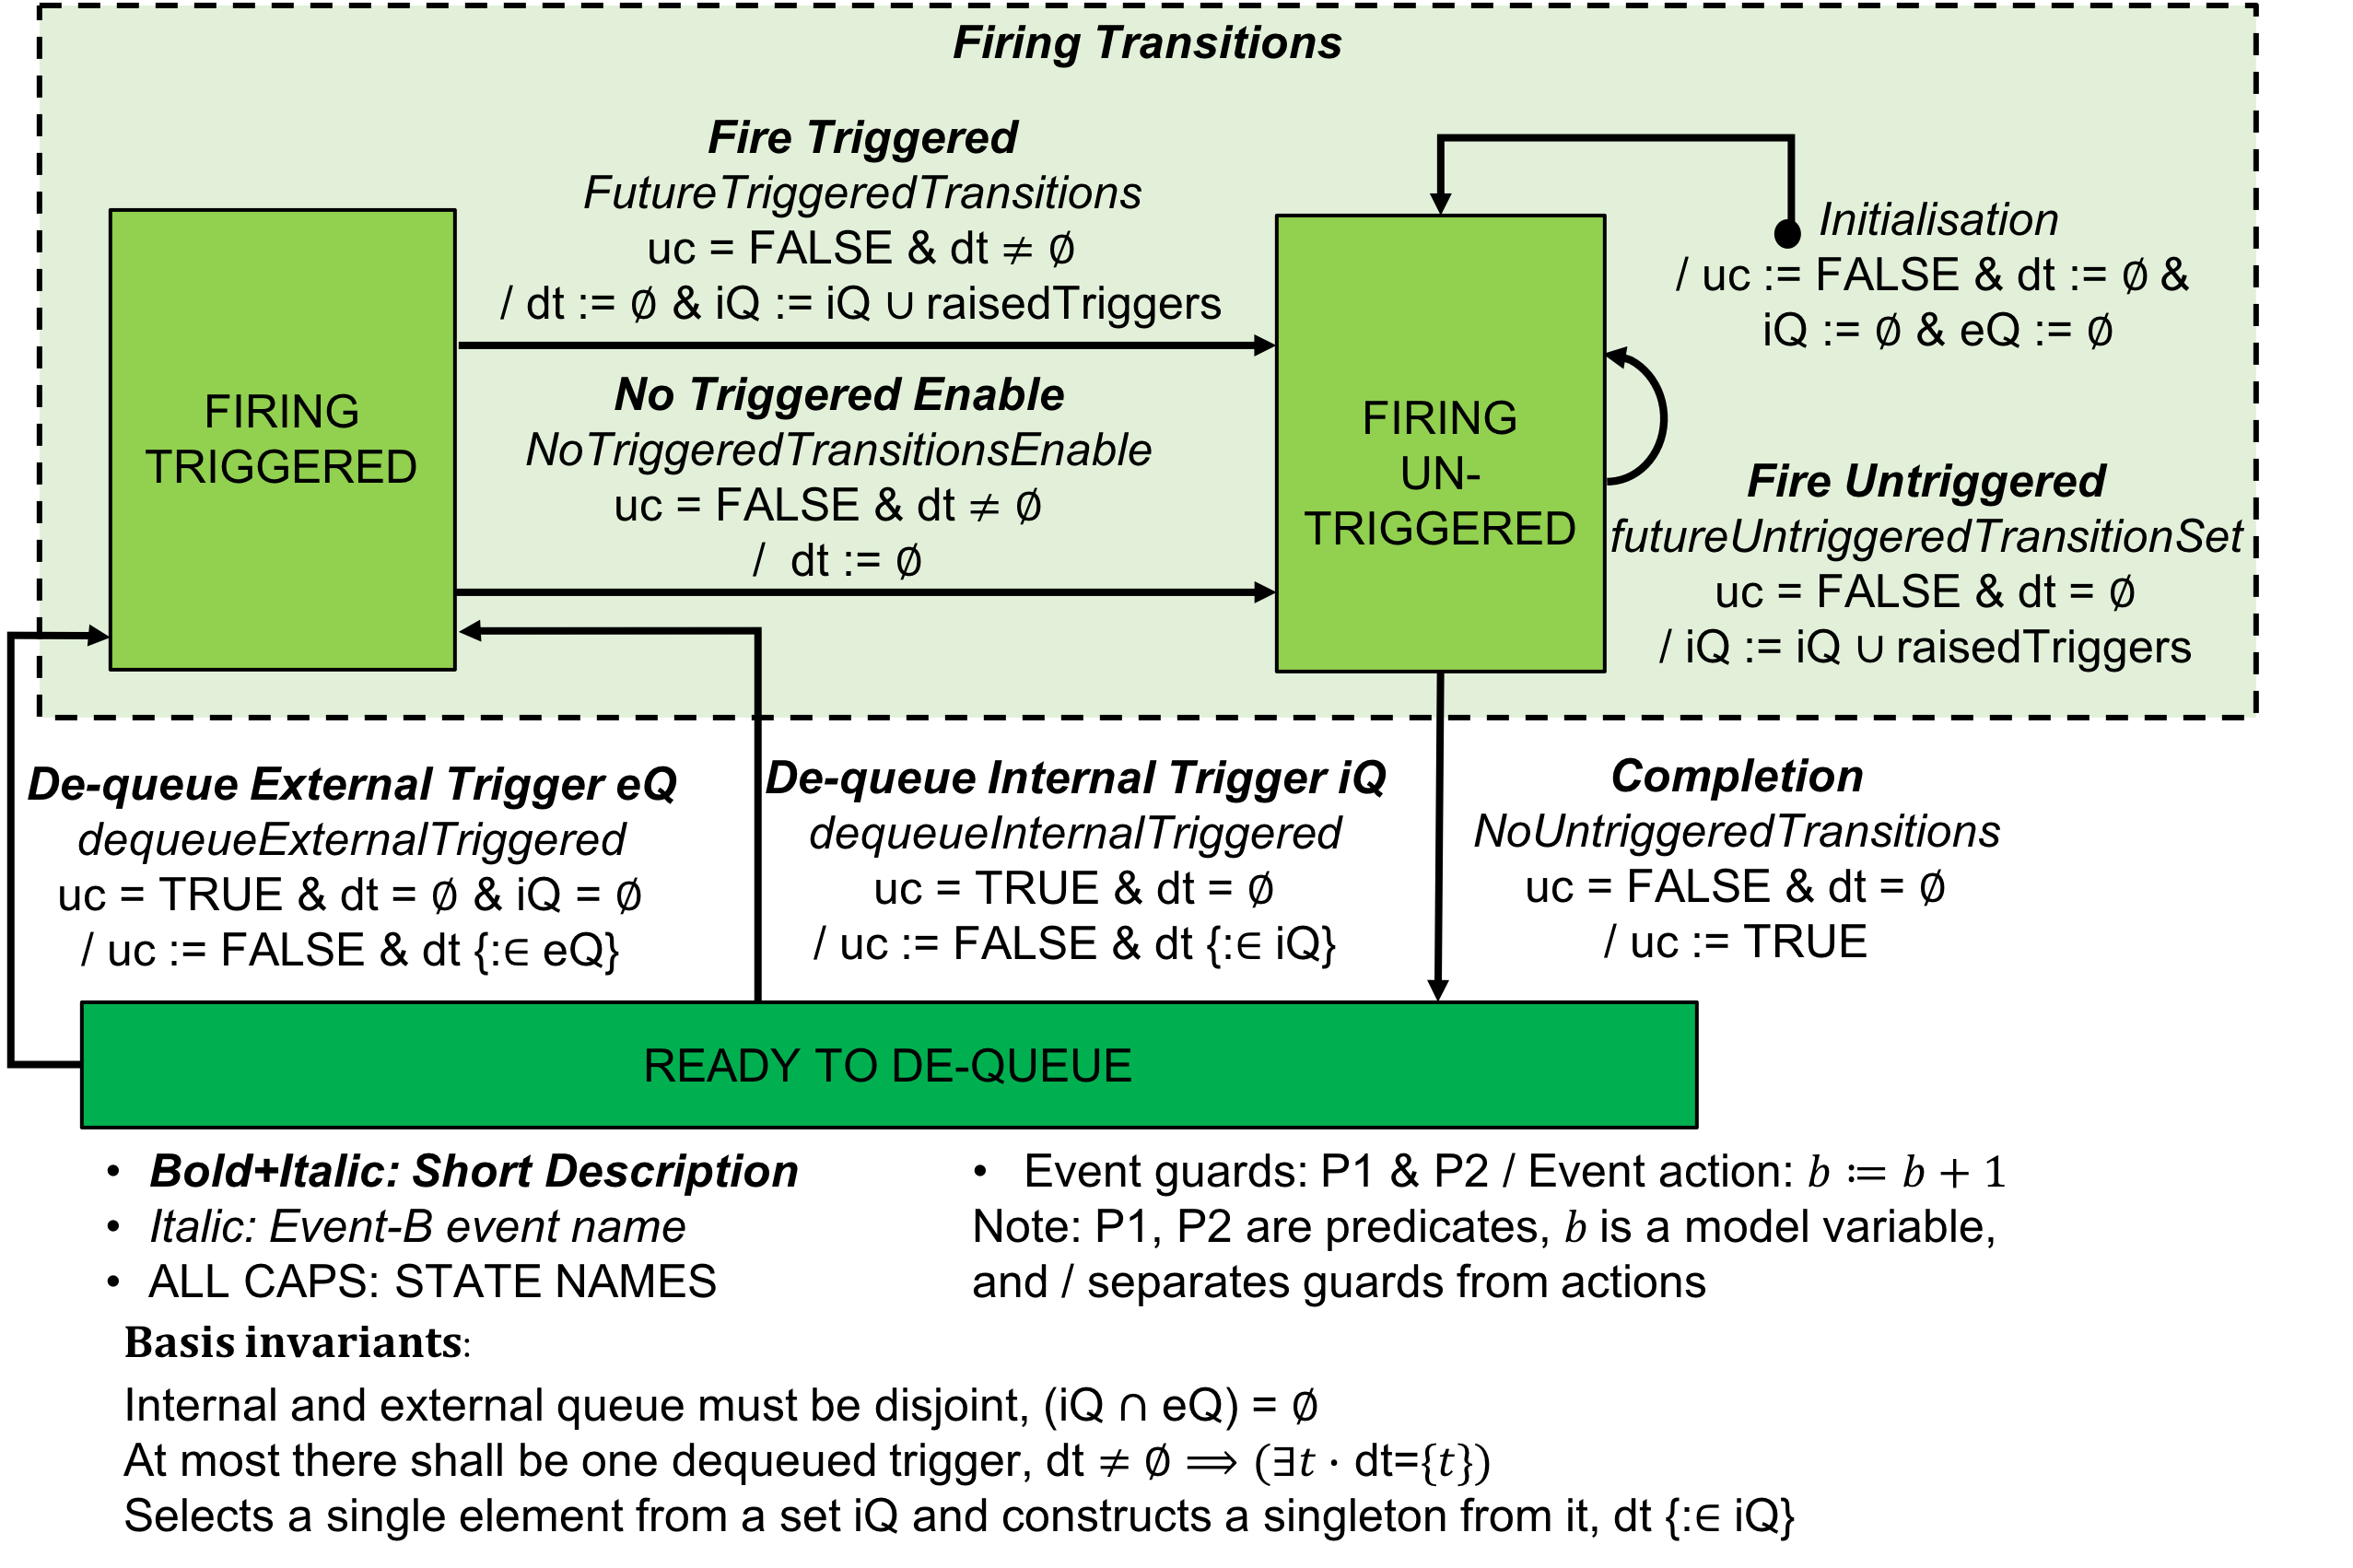
\includegraphics[width=0.90\textwidth, trim=30 50 60 0]{figures/Picture6.png}
	\caption{Abstract representation of run to completion basis}
	\label{fig:basis}
	\vspace{-.4cm}
\end{figure}

The specification of this basis consists of an \EVENTB \emph{context} and \emph{machine} that are the same for all input models and are refined by the specific output of the translation.  
The basis context, shown in listing \ref{lst:BasisContext}, introduces a set of all possible triggers, |SCXML_TRIGGER| which is partitioned into internal and external triggers 
(e.g |FutureInternalTrigger| and |FutureExternalTrigger| respectively), 
some of which will be introduced in future refinements. 
At each refinement these trigger sets are further partitioned to introduce more concrete triggers, 
leaving a new abstract set to represent the remaining triggers yet to be introduced. 

The context also models \emph{sequences} of triggers as a data type to be used for the trigger queues.
Our initial work modelled queues abstractly as sets of triggers which was adequate for most verification purposes but does not enforce fairness on trigger consumption~\cite{MoSnHo18,MoSnHo-ABZ2020,detect2020}. 
Hence we were forced to introduce fairness assumptions regarding trigger consumption in order to verify liveness properties.
In this paper we introduce sequences to properly model the trigger queues which are an implementation of this fairness property. 
Note that the queue also enables the same trigger to be raised twice in the queue which was not possible in a set.
The constant |Seq| returns the set of all possible sequences of a given subset of triggers and is defined using lambda calculus.
Constant functions are also defined for the usual operations on sequences: 
\emph{length} of a given sequence, 
\emph{append} a trigger to the end of a sequence to give a new sequence, 
\emph{concat}enate two sequences to give a new sequence, 
return the trigger at the \emph{head} of a sequence, 
return the sequence that makes up the \emph{tail} of a sequence and 
return the \emph{content} (set of triggers) involved in a sequence. 
The Basis context also defines several theorem properties about sequences that are needed to discharge proof obligations.
These are omitted from Listing~\ref{lst:BasisContext} for brevity.

\ColinInlineComment{I changed the comments to a command in order to get them to align.  Is there a better way? }
\newcommand*{\Comment}[1]{\color{green!50!black}\hfill\makebox[0.6\textwidth][l]{#1}}%

 \begin{lstlisting}[caption={Abstract basis context},label={lst:BasisContext}, language=Event-B, tabsize=8, escapechar=€, frame=single, basicstyle=\rmfamily\scriptsize, belowskip=-2.0 \baselineskip, float=t]
 context
 	basis_c 	€\Comment{// (generated for SCXML)}€
 sets
 	SCXML_TRIGGER	 €\Comment{// all possible triggers}€
 constants
 	FutureInternalTrigger	€\Comment{// all possible internal triggers}€
 	FutureExternalTrigger	€\Comment{// all possible external triggers}€
 	Seq							€\Comment{// return all possible sequences of given set of triggers}€
 	Seq_length					€\Comment{// return the length of a sequence of triggers}€
 	Seq_append					€\Comment{// return the result of appending trigger to a sequence}€
 	Seq_concat					€\Comment{// return the concatenation of two sequences of triggers}€
 	Seq_head					€\Comment{// return the trigger at head of a sequence of triggers}€
 	Seq_tail					€\Comment{// return the sequence at tail of a sequence of triggers}€
 	Seq_content					€\Comment{// return the set of triggers in a sequence of triggers}€
 	InternalQueueType			€\Comment{// type of internal queues}€
 	ExternalQueueType			€\Comment{// type of external queues}€
 	
 axioms
 	partition(SCXML_TRIGGER, FutureInternalTrigger, FutureExternalTrigger) 
 	Seq = (λT · T ⊆ SCXML_TRIGGER ∣ {n, s · n ∈ ℕ ∧ s ∈ 0 ‥ n − 1 → T ∣ s})
 	Seq_length = (λs · s ∈ Seq(SCXML_TRIGGER) ∣ card(s))
 	Seq_append = (λ s ↦ t · s ∈ Seq(SCXML_TRIGGER) ∧ t ∈ SCXML_TRIGGER ∣ 
 		{i↦v ∣ i ∈ 0 ‥ Seq_length(s) ∧ (i < Seq_length(s) ⇒ v = s(i)) ∧ (i = Seq_length(s) ⇒ v = t) } )
	Seq_concat = (λ s1 ↦ s2 · s1 ∈ Seq(SCXML_TRIGGER) ∧ s2 ∈ Seq(SCXML_TRIGGER) ∣ 
		{i↦v ∣ i ∈ 0 ‥ Seq_length(s1) + Seq_length(s2) − 1 ∧ (i < Seq_length(s1) ⇒ 
									v = s1(i)) ∧ (i ≥ Seq_length(s1) ⇒ v = s2(i − Seq_length(s1))) } )
	Seq_head = (λs · s ∈ Seq(SCXML_TRIGGER) ∧ s ≠ ∅ ∣ s(0))								
	Seq_tail = (λs· s∈Seq(SCXML_TRIGGER) ∧ s≠∅ ∣ {i↦v ∣ i∈0‥Seq_length(s)−2 ∧ v=s(i+1)} )	
	Seq_content = (λs · s ∈ Seq(SCXML_TRIGGER) ∣ ran(s))
	InternalQueueType = Seq(FutureInternalTrigger)
	ExternalQueueType = Seq(FutureExternalTrigger)
 end
 \end{lstlisting}	

Each of the transitions in the basis (see Figure~\ref{fig:basis}) represents an abstract event of the basis machine (Listing~\ref{lst:BasisMachine}) that describes the generic behaviour of models under a run to completion semantics.
These events provide an abstraction that defines the altering of trigger queues and completion flag. 
\EventB refinement rules prohibit new events from modifying abstract variables (i.e. new events refine `skip').
Hence, since \SCXML transitions need to modify the trigger queues etc., used to capture the \SCXML run to completion semantics, all events generated by translation of the specific \SCXML model,  must refine abstract events introduced for this purpose in the basis.
The basis machine also declares variables that correspond to the currently dequeued trigger,  |dt|, 
the queue of internal triggers raised by actions within the model, |iQ|, 
the queue of external triggers raised by the environment, |eQ|,
and a flag, |uc|, that signals when a run to completion macro-step has been completed 
(no un-triggered transitions are enabled). 
Note that, for convenience, the currently dequeued trigger, |dt|, is modelled as a singleton set which may be empty (i.e. consumed) or contain the single trigger to be consumed.

The trigger queues and dequeued trigger are initialised to empty and |uc| is set to |FALSE| so that any enabled un-triggered transitions are dealt with via the |futureUntriggeredTransitionSet| event when the system first starts (see Listing~\ref{lst:scxml-r2c}).
This will subsequently enable completion and reset the |uc| flag to |TRUE|.
The abstract event |futureRaiseExternalTrigger| represents the raising  of an external trigger (not shown in figure~\ref{fig:basis}).    
After completion, a queued trigger can be prepared for consumption by moving it to the dequeued trigger, |dt|.
Internal triggers have a higher priority, since the external trigger queue is only dequeued if the |iQ| is empty (see |dequeueExternalTriggered| and |dequeueInternalTriggered| in Figure~\ref{fig:basis}).
The abstract event |futureTriggeredTransitionSet| represents a combination of parallel transitions that may be simultaneously triggered by the dequeued trigger, |dt|.
When the actual example \SCXML is translated, a separate refinement of this abstract event will be generated for each subset of the set of parallel transitions that could fire in parallel in order to cater for all possibilities of enablement, however, as the model is refined some combinations may be eliminated as the guards are strengthened.
This approach to generating an event for each possible combination of each set of transitions that could fire in parallel is needed because of the batch enabling semantics of the SCXML run to completion (see Section~\ref{sec:scxml}).
The actions of these transitions may also raise triggers of their own in the internal trigger queue |iQ|.


Completion of triggered and untriggered transitions may be non-deterministically premature to allow future refinements to strengthen the guards of transitions (i.e. to disable them resulting in an earlier completion).
In the process of refining a model, a designer takes advantage of this non-determinism in the abstraction by adding nested sub-states and explicit guards to transitions. 
When a refinement level is reached where the designer wants to enforce a requirement (i.e. prevent it being bypassed by a non-deterministic completion), the model needs to be \emph{finalised} (see Section~\ref{sec:translation} for more on finalisation). 
The \SCXML translation tool will then automatically strengthen the guards of events |noTriggeredTransitionsEnabled| and |noUntriggeredTransitionsEnabled|, to ensure that the run to completion sequence is not interrupted by non-deterministic behaviour. 
To do this we need to guard completion so that it cannot happen while any relevant transition is still enabled.
To finalise a triggered transition, the guard of |noTriggeredTransitionsEnabled| is strengthened by adding the conjunction of the negated guards of all transitions that can fire in parallel with the transition being finalised.
%(To fire in parallel a transition must be in a parallel region of the state-chart and be triggered by the same trigger).
Similarly, to finalise an untriggered transition, the guard of |noUntriggeredTransitionsEnabled| is strengthened by adding the conjunction of the negated guards of all untriggered transitions that can fire in parallel.
It may seem that finalisation could cause an unmanageable explosion of guards.
However, to fire in parallel, transitions must be contained in parallel regions and also be enabled by the same trigger (or be un-triggered).
In practice, since most systems do not contain many parallel regions, the number of transitions that can fire in parallel is limited.
Transition finalisation can be left until it is needed for the proof of a particular property and does not generate any new proof obligations since adding guards is a trivial refinement step.
Finalisation is also needed in order to remove non-deterministic behaviours when the model is animated for validation purposes.

% The basis machine declares variables 
% that correspond to the triggers present in the queue at any given time, and a flag, |SCXML_uc|, that signals when a run to completion macro-step has been completed (no un-triggered transitions are enabled). 
% After initialisation, both trigger queues are empty and |SCXML_uc| is set to |FALSE| so that un-triggered transitions are dealt with. 
% The basis machine provides events that describe the generic behavior of models that follow the run to completion semantics in terms of altering the trigger queues and completion flag.
% Since new events introduced in a refinement cannot modify existing variables, all future events generated by translation of the specific \SCXML model, will refine these abstract events.
% The abstract event, |SCXML_futureRaiseExternalTrigger| represents the raising of an external trigger (this transition is not shown in the diagram).    
% The abstract event, |SCXML_futureInternalTransitionSet| represents a combination of transitions that are triggered by an internal trigger. 


% The guards of this event ensure prior completion of the previous macro-step. 
% A similar event, |SCXML_futureExternalTransitionSet| (not shown) represents a combination of transitions that are triggered by an external trigger and has the additional guard that the internal trigger queue is empty.
% These two triggered transition events reset the completion flag to ensure that any un-triggered transitions that may have become enabled have a chance to fire next.
% The abstract event |SCXML_futureUntriggeredTransitionSet| represents a combination of transitions that are un-triggered and may only be fired when the completion flag is unset (FALSE).
% It leaves the completion flag unset in case further combinations of un-triggered transitions are enabled.
% All three of these transition events also allow for raising a non-deterministic set of internal triggers.
% A final abstract event, |SCXML_completion|, sets the completion flag (TRUE) if it is not already set. At this abstract basis level, this is non-deterministically fired since we do not yet have any detail of what needs to be completed.




 \begin{lstfloat}[!tb]
 \begin{lstlisting}[caption={Abstract basis machine}, label={lst:BasisMachine},language=Event-B, escapechar=€, frame=single, basicstyle=\rmfamily\scriptsize, belowskip=-2.0 \baselineskip]
 MACHINE	basis	   €\Comment{//   (generated for SCXML)}€
 SEES    	basis_ctx
 VARIABLES
 €~~€	iQ	   €\Comment{//   internal trigger queue}€
 €~~€	eQ	   €\Comment{//   external trigger queue}€
 €~~€	uc	   €\Comment{//   run to completion flag}€
 €~~€	dt	   €\Comment{//   dequeued trigger for this run}€
 INVARIANTS
 €~~€	iQ ∈ InternalQueueType	   	€\Comment{//   internal queue}€
 €~~€	eQ ∈ ExternalQueueType	   	€\Comment{//   external queue}€
 €~~€	uc ∈ BOOL	   				€\Comment{//   completion flag}€
 €~~€	dt ⊆ SCXML_TRIGGER	   		€\Comment{//   dequeued trigger}€
 €~~€	dt≠∅ ⇒(∃t·dt={t})			€\Comment{//   at most one dequeued trigger}€
 EVENTS
 	INITIALISATION   €\Comment{// queues empty, completion false, no dequeued triggers}€
 			iQ, eQ, uc, dt ≔ ∅,	∅, FALSE, ∅  
 	END

 	futureRaiseExternalTrigger      	   €\Comment{//basis of future event to raise an external trigger}€
 		ANY 	raisedTrigger	WHERE raisedTrigger ∈ FutureExternalTrigger
 		THEN	eQ≔append(eQ ↦ raisedTrigger)
 	END

 	dequeueInternalTrigger      	   €\Comment{//event to dequeue an internal trigger}€ 
 		WHEN	iQ≠∅ & dt=∅ & uc=TRUE 
 		THEN	dt, iQ, uc ≔ {head(iQ)}, tail(iQ), FALSE
 	END

 	dequeueExternalTrigger      	   €\Comment{//event to dequeue an external trigger}€ 
 		WHEN	eQ≠∅ & dt=∅ & uc=TRUE & iqQ∅
		THEN	dt, eQ, uc ≔ {head(eQ)}, tail(eQ), FALSE
 	END

 	futureTriggeredTransitionSet      	€\Comment{//basis of future event representing triggered transitions}€
 		ANY trigger, raisedTriggers WHERE trigger ∈ dt & uc = FALSE & raisedTriggers ∈ Seq(FutureInternalTrigger)
 		THEN	dt, iQ ≔ ∅ , concat(iQ↦raisedTriggers)
 	END

 	noTriggeredTransitionsEnabled      	€\Comment{//event to fire when no triggered transitions enabled}€ 
 		WHEN 	uc=FALSE & dt≠∅
 		THEN	dt ≔ ∅
 	END

 	futureUntriggeredTransitionSet      €\Comment{//basis of future event representing untriggered transitions}€
 		ANY	raisedTriggers	WHERE	uc=FALSE & dt=∅ & raisedTriggers∈Seq(FutureInternalTrigger)
 		THEN iQ ≔ concat(iQ↦raisedTriggers)
 	END

 	noUntriggeredTransitionsEnabled      €\Comment{//event fired when no untriggered transitions enabled}€
 		WHEN	uc=FALSE & dt=∅
 		THEN	uc ≔ TRUE
 	END
 END
 \end{lstlisting}
 \end{lstfloat}

% \begin{lstfloat}[!tb]
% \begin{lstlisting}[caption={Event-B event corresponding to internal triggered transition to \textbf{Wait50ms} state in refinement level 1 shown in Fig.~\ref{fig:ASIC}}, label={lst:SecBotMach0},language=Event-B, escapechar=|, frame=single, belowskip=-2.0 \baselineskip]
% spi_done__InitialiseSensor_Wait50ms:	
% refines SCXML_futureInternalTransitionSet 
% any SCXML_it SCXML_raisedTriggers where
% SCXML_it  ∈ SCXML_iq 
% SCXML_uc = TRUE
% SCXML_raisedTriggers ⊆ SCXML_FutureInternalTrigger
% InitialiseSensor = TRUE
% SCXML_it = spi_done  	//trigger for this transition |\label{line:defTrigger}|
% then
% SCXML_uc ≔ FALSE
% SCXML_iq ≔ (SCXML_iq ∪ SCXML_raisedTriggers) ∖ {SCXML_it}
% InitialiseSensor ≔ FALSE
% Wait50ms ≔ TRUE
% end
% \end{lstlisting}
% \end{lstfloat}

%%% Local Variables:
%%% mode: latex
%%% TeX-master: "../main"
%%% End:

% !TEX root = ../main.tex
\section{Description of the Sample Application}
\label{sec:descr-sample-appl}

To illustrate the development and analysis process of a design using the previously described 
state-chart semantics, we will discuss a quadrotor helicopter or quadrotor application similar to 
the one presented by Syriani et al.~\cite{Syriani_2019}. 
The application will focus on the incremental design of some of the drone's required functionality.
The constructed model must obey state-chart refinement rules listed in Section~\ref{sec:intro}, these rules are proven within the Rodin tool.
The structure of the state-chart for this model at each subsequent abstraction level restricts further the development of the model to refinements that obey the rules. 
This will allow us to prove properties of the model in a very strategic fashion, as properties proven of early abstraction levels are preserved in later refinements.

The initial abstraction and first refinement of the model, shown in Figure~\ref{fig:drone1}, capture the basic functionality of the drone. 
The abstract model is shown in blue; the model's initial state is |OFF| and as a result of the |on| and  |toTakeoff| external triggers it transitions to the |START| and |OPERATIONAL| states respectively\footnote{Transitions in Figures~\ref{fig:drone1}--\ref{fig:drone4} are labeled with trigger names
(e.g. toTakeoff, toFly) not with event names as it is in \UMLB.}. 
The drone reacts to the |off| external trigger by shutting down and subsequently transitioning to the |OFF| state.
The first refinement is constructed using \emph{Rule C}, which adds details within the |OPERATIONAL| state (gray states in Figure~\ref{fig:drone1}).
Within the |OPERATIONAL| state the drone will transition to |FLY| or |DESCEND| after the internal trigger |toFly| or |toLand| is raised, respectively. 
In refinement level one, these internal triggers are raised non-deterministically in the system by functionality not currently defined.
As additional details are incorporated into the model in later refinements some of that non-determinism is 
removed and replaced by transitions with actions that raised the previously defined internal triggers.
A further external trigger, |landed|, directs the system to progress to the |LANDED| state.
It should be noted that this abstraction of the drone model includes a transition from |TAKEOFF| to |DESCEND| (dashed transition in Figure~\ref{fig:drone1}). 
This allows for the drone to respond to a |toLand| trigger if it encounters some problems while in the |TAKEOFF| state.
Syriani et al.~\cite{Syriani_2019} introduces this transition in later refinements under Rule 8 \emph{path refinement rule}. 
This rule is inconsistent with our rules of refinement as it results in a concrete event with no corresponding behavior in the abstraction.

% \begin{figure}[!h]
\begin{figure}[]
	\vspace{-.4cm}
	\centering
	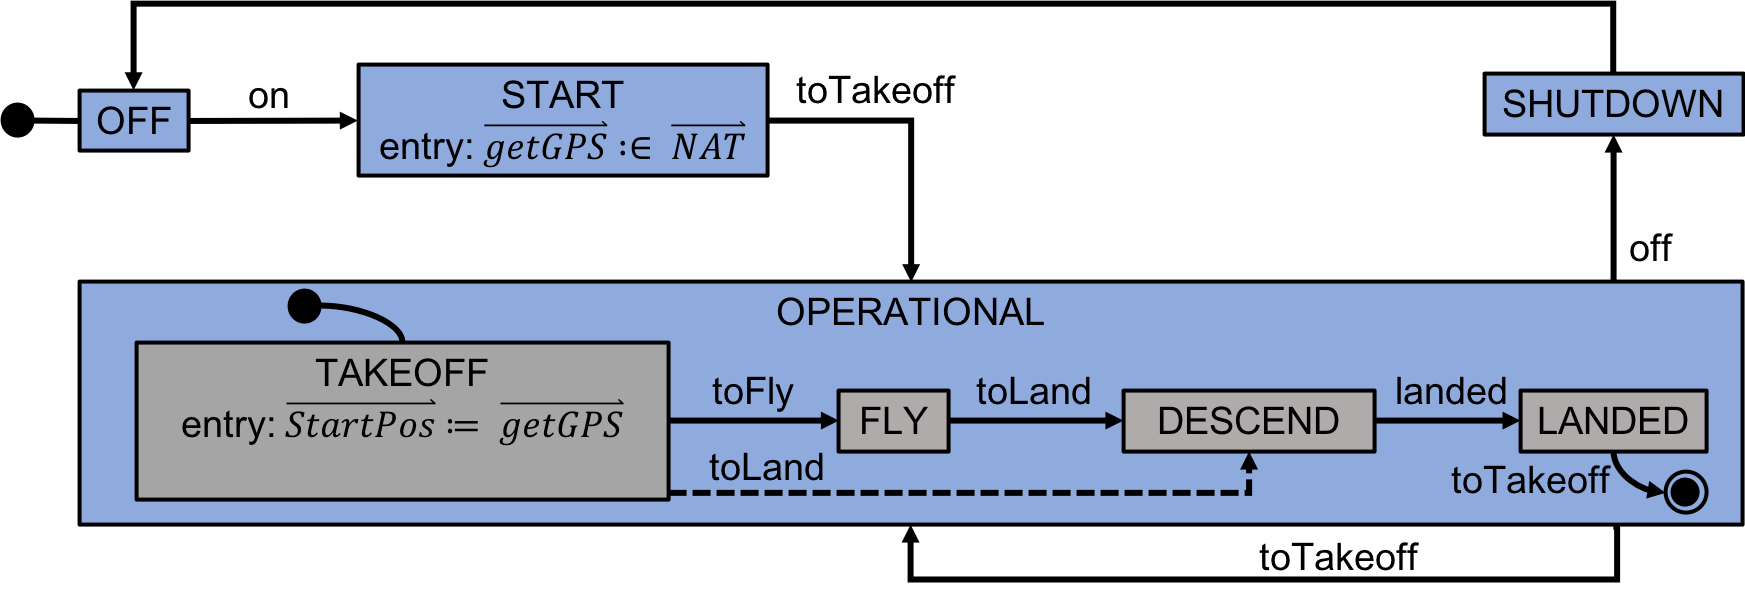
\includegraphics[width=0.90\textwidth, trim=0 40 0 0]{figures/Picture1.png}
	\caption{State-chart of drone application. Abstract level including only generic start/shutdown behavior (shown in blue). The first refinement introducing main operational sub-states, is shown in gray. }
	\label{fig:drone1}
	\vspace{-.4cm}
\end{figure} 


% Figure~\ref{fig:drone2} shows the first refinement of the model, as we refine the parent state |TAKEOFF|
% by introducing child states and new model variables, similar to 
% Rule 2 \emph{basic-to-or state rule} defined by Syriani et al.~\cite{Syriani_2019}
% As part of this refinement we introduced an untriggered transition responsible for 
% raising the |toFly| internal trigger, and therefore removed some of the non-determinisms in the abstraction.

% \begin{figure}[!h]
% 	\centering
% 	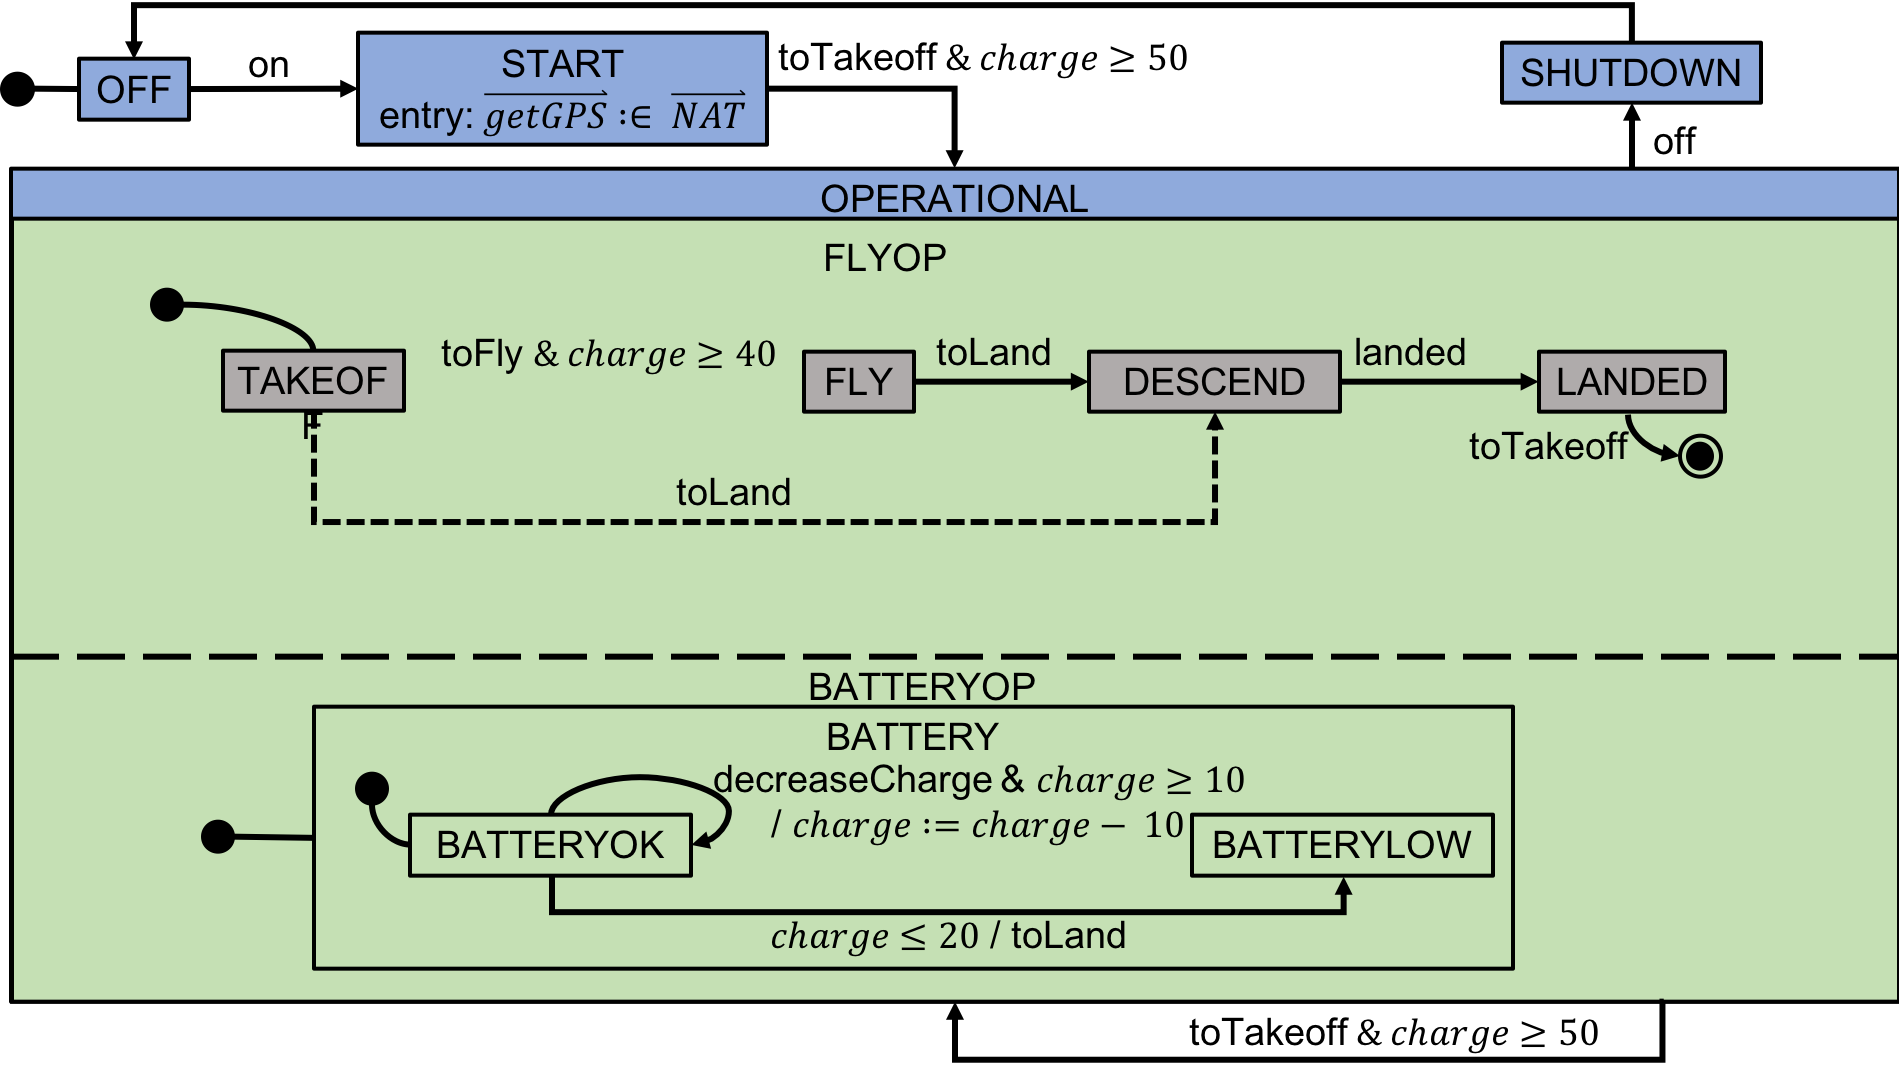
\includegraphics[width=0.95\textwidth]{figures/Picture2.png}
% 	\caption{State-chart of drone application. Refinement level introducing details for take off.}
% 	\label{fig:drone2}
% \end{figure} 
% \begin{figure}[!h]

\begin{figure}[]
	\centering
	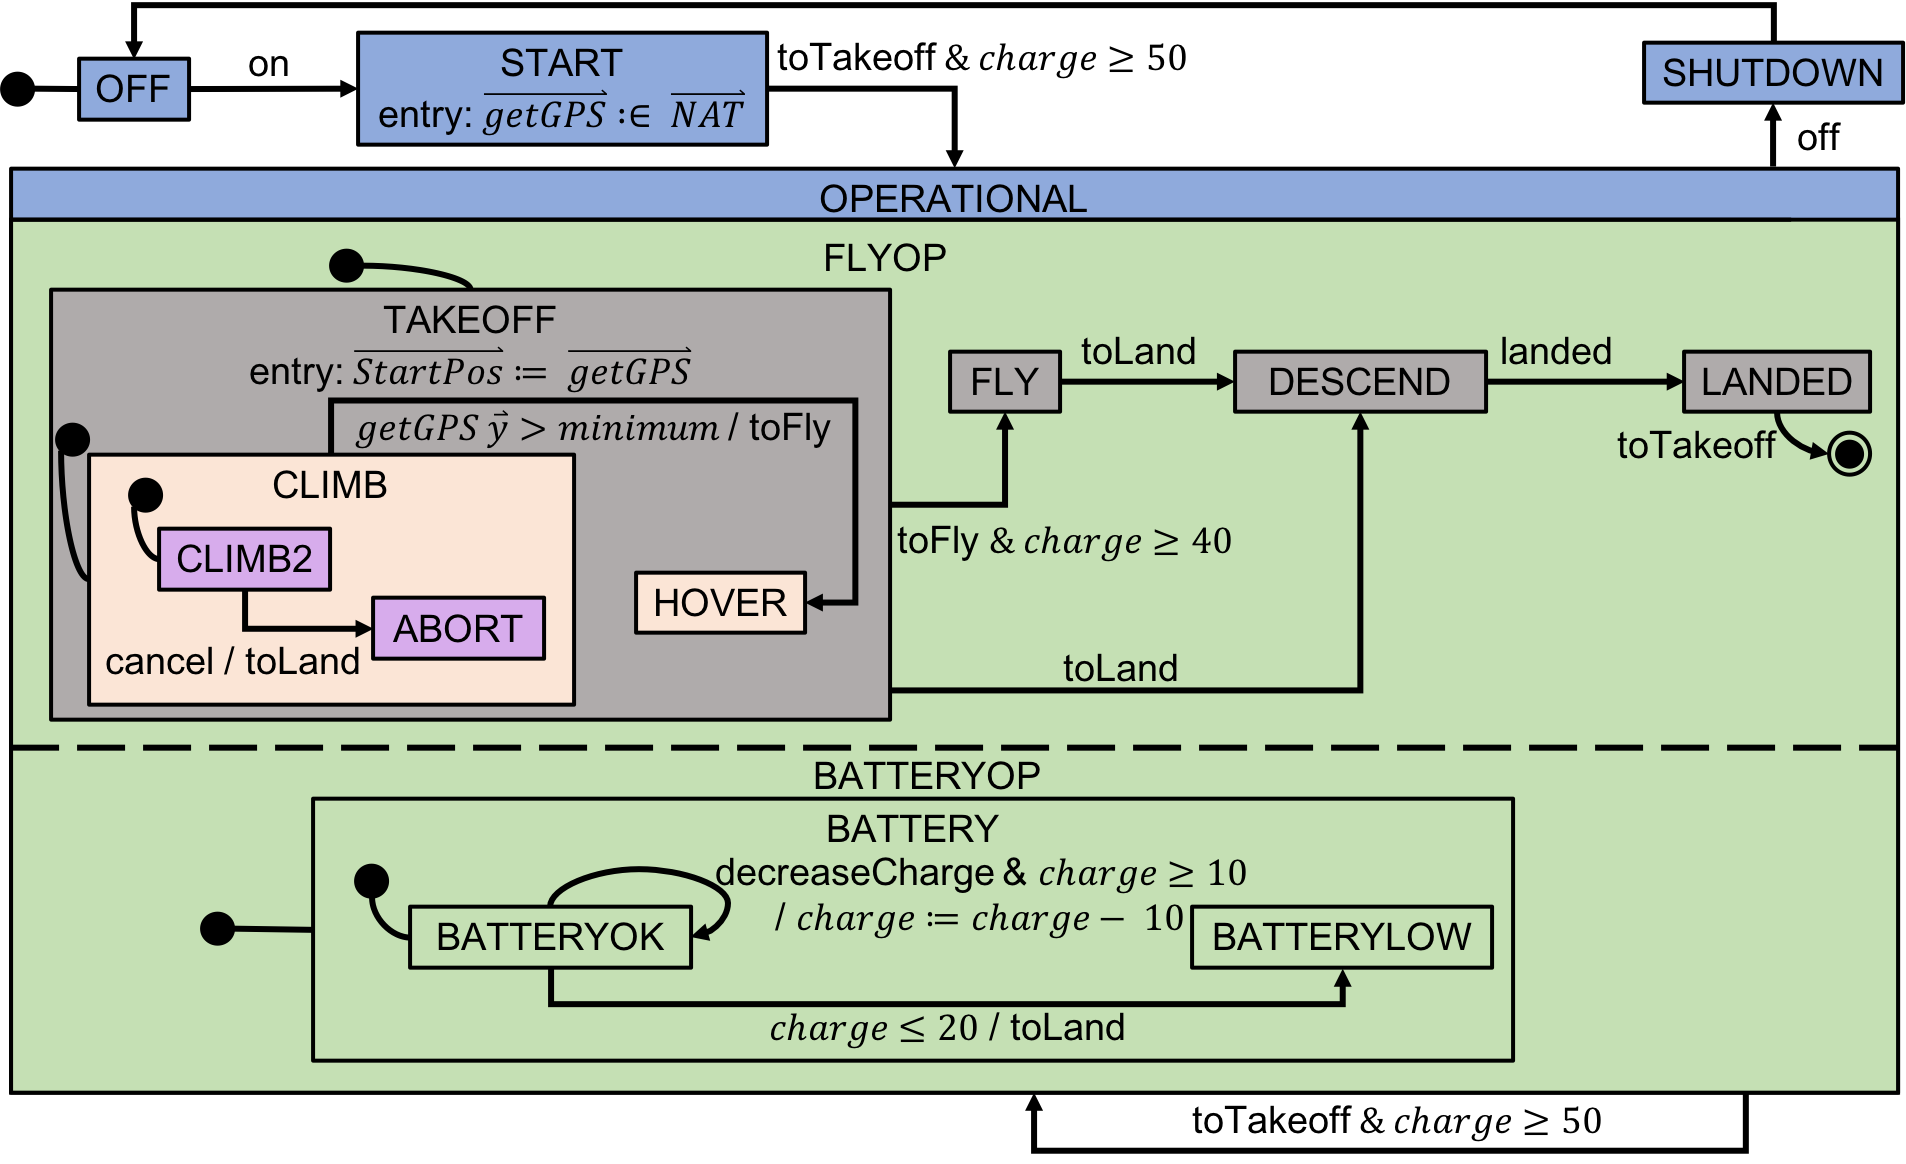
\includegraphics[width=0.90\textwidth, trim=0 30 0 0]{figures/Picture5.png}
	\caption{State-chart of drone application. 
		2nd refinement for battery monitoring functionality (shown in green).
		3rd refinement introducing details for take off (shown in beige).
		4th refinement level to allow cancelling during take-off (shown in lilac).}
	\label{fig:drone4}
\end{figure} 

Figure~\ref{fig:drone4} builds on Figure~\ref{fig:drone1} to show three more refinements to the drone model. 
% Figure~\ref{fig:drone4} shows two subsequent refinements to the drone model.
The second refinement (shown in green in Figure~\ref{fig:drone4}) extends the capabilities within |OPERATIONAL| by using \emph{Rule C} to make it a parallel state that controls flying and battery related functionality. 
This is the same as Rule 4 \emph{and-state rule} defined by Syriani et al.~\cite{Syriani_2019}.
The charge within the drone battery is monitored by the parallel |BATTERYOP| state. 
A new ancillary variable, |charge|, is introduced to keep track of the amount of charge left in the drone.
It is decreased by a self-transition on state |BATTERYOK| in response to an external trigger |decreaseCharge|. 
%As part of this design stage we introduce a requirement to constrain drone flying operation to a battery charge of at least 20\% capacity.
If the battery monitor works correctly we would expect the battery charge to have at least 20\% capacity while in the state |BATTERYOK|.
This can be expressed as an invariant property:
\begin{center}
	|(BATTERYOK = TRUE) => charge > 20|\% .
\end{center}
When the monitored charge drops to 20\% or less, the |BATTERY| state-chart raises the internal trigger |toLand|, which will cause a reaction in the |FLYOP| start-chart to bring it out of |TAKEOFF| or |FLY| and into |DESCEND| (hence removing some of the non-determinism concerning where |toLand| is raised).
While in the |TAKEOFF| state we would expect the battery monitor to be in the |BATTERYOK| state or to have raised a |toLand| trigger.
\begin{center}
	|(TAKEOFF = TRUE) => (BATTERYOK = TRUE ∨ toLand)|~.
\end{center}
%The aforementioned trigger, is raised non-deterministically by some unspecified internal functionality .
%Our state-chart semantics supports transition refinement, which allows us to modify previously defined transitions, by adding guards \emph{Rule A} and/or actions \emph{Rule B} that modify new variables that contribute implementation details to the model. 
To ensure the drone only enters |TAKEOFF| or |FLY| with enough battery power we strengthen the guards of transitions to the |FLY| and |TAKEOFF| states (\emph{Rule A}).
We will discuss how these state invariant properties are verified in Section~\ref{sec:verificationSafety}.

% \begin{figure}[!h]
% 	\centering
% 	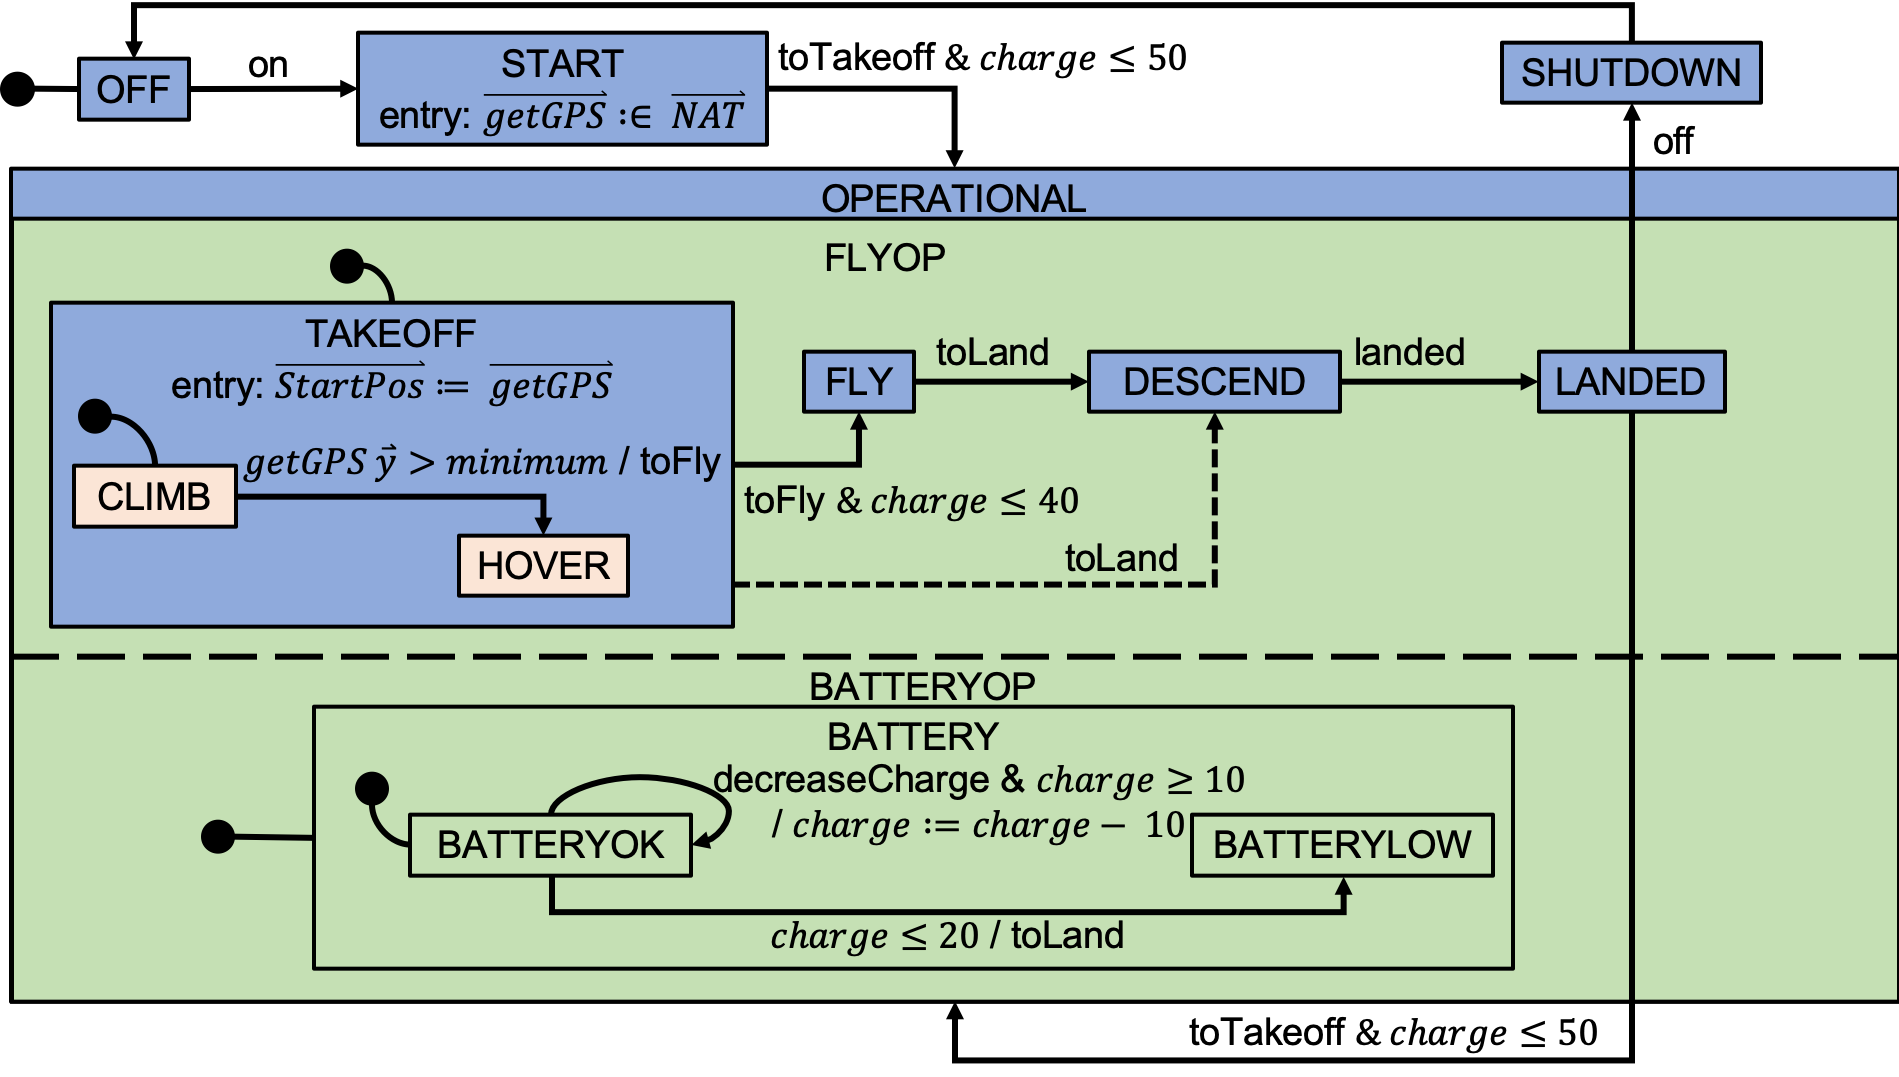
\includegraphics[width=0.95\textwidth]{figures/Picture3.png}
% 	\caption{State-chart of drone application.Refinement level for descending capabilities}
% 	\label{fig:drone3}
% \end{figure} 

The third refinement of the model (shown in beige) refines the state |TAKEOFF| by applying \emph{Rule B and C}. 
Under these rules we introduce child states and new model variables, similar to Rule 2 \emph{basic-to-or state rule} defined by Syriani et al.~\cite{Syriani_2019}
As part of this refinement we introduced an untriggered transition responsible for raising the |toFly| internal trigger, and therefore removed some of the non-determinisms concerning this trigger.

The fourth refinement of the drone model (shown in lilac) uses \emph{Rule C} to introduce additional implementation details to 
allow a take-off to be cancelled in response to an external trigger |cancel|.
%ensure that under special 
%circumstances (e.g. sensing of adverse environment or unexpected battery dropped) the drone is able 
%to circumvent flying and proceed to an emergency landing. The previously described requirement can be
%expressed as
%\begin{center}
%  |(TAKEOFF = TRUE) => (BATTERYOK = TRUE ∨ toLand)|~.
%\end{center}
%To implement this new capability in the design the internal trigger |cancel| is introduced.
%The internal trigger |cancel| can be raised non-deterministically by some sensing capability, 
%the details of which are not currently implemented. 
If the trigger is raised, the climbing process must be aborted and the drone descending sequence shall start. 
This refinement level is done differently to Syriani et al.~\cite{Syriani_2019}, which follows Rule 7 \emph{state extension rule}. 
The aforementioned rule requires a data remapping of the abstract states |TAKEOFF|, |CLIMB| and |HOVER|, which should be distinct from the states in this  refinement, as the state |ABORT| is introduced.
In contrast, we implement this refinement using a rule similar to Syriani et al.'s  Rule 2 \emph{basic-to-or state rule}, which introduces the concrete states |CLIMB2| and |ABORT| to the abstract state |CLIMB|.


% Syriani et al. refinement rules
% Rule 1 \emph{action rule}
% Rule 2 \emph{basic-to-or state rule}
% Rule 3 \emph{or-to-and state rule}
% Rule 4 \emph{and-state rule}
% Rule 5 \emph{transition rule}
% Rule 6 \emph{fork rule}
% Rule 7 \emph{state extension rule}
% Rule 8 \emph{path refinement rule}

% Event-B refinement rules
% https://www3.hhu.de/stups/handbook/rodin/current/html/generated_proof_obligations.html
% guard strengthening
% action simulation
% equality of a preserved variable
% guard strengthening (merge)
% well definedness of a witness
% feasibility of witness
% decreasing of variant

%%% Local Variables:
%%% mode: latex
%%% TeX-master: "../main"
%%% End:

% !TEX root = ../main.tex

\section{\SCXML Translation to \UMLB/\EventB}
\label{sec:translation}

The translation of a specific \SCXML model to \UMLB and  \EventB, comprises the following stages: 
\begin{itemize}
	\item 
Firstly, a basis machine and context are created to embody the semantics of the \SCXML language (as described in Section~\ref{sec:run-completion}).
The basis provides variables and events to model the queue of triggers as well as abstract versions of events to model transitions firing.
The basis is independent of the particular \SCXML model which is added in subsequent refinements.
Hence it is not necessary to re-prove any of the proof obligations associated with this basis.
	\item 
Secondly, all possible combinations of each set of transitions that can fire together are calculated and corresponding events are generated, at appropriate refinement levels (given by the refinement annotations embedded in the \SCXML model), that refine the abstract basis events.
The transitions that can fire together are those that are triggered by the same trigger (or are both untriggered) and are in different parallel (`and') sub-states.
If these transitions raise internal triggers, a guard, |{i1, i2, ...} <: content(raisedTriggers)| (where |i1, i2, ...| have been added to the internal triggers set), is introduced to define the raised triggers parameter. 
The subset used in the guard retains non-determinism to allow more triggers to be raised in later refinements.
For triggered transitions, the trigger is specified by a guard that defines the value of the trigger parameter. 
	\item 
Thirdly, at each refinement level, the \SCXML state-chart is translated into a corresponding \UMLB state-machine whose transitions elaborate (i.e. add state change details to) the transition combination events that the transition may be involved in.
A transition may fire in parallel with transitions of parallel nested state-machines that have the same (possibly null) trigger.
	\item
Finally the \UMLB state-machine is translated into \EVENTB by programmatically invoking the \UMLB translator.
\end{itemize}

% Further details of the translation are given in~\cite{MoSn16,MoSnHo18,MoSnHo-ABZ2020}.

 A previous version of the translator was described in ~\cite{MoSnHo18} New features of the translation added since~\cite{MoSnHo18} are as follows:
 \begin{description}
 \item[Trigger queues in basis:]
 	\begin{sloppypar}
 		The encoding of trigger queues in the abstract basis context and machine has been improved so that a queue is properly modelled as a sequence of triggers.
 		This more accurately reflects the \SCXML semantics.
 	\end{sloppypar}
 \item[Dequeing triggers from queues:]
   \begin{sloppypar}
     The abstract basis machine has been improved so that triggers are properly dequeued before potential use,
     which allows triggers to be discarded if the controller cannot respond to them. 
     This more accurately reflects the \SCXML semantics and was necessary in order to model the new drone case study properly.
   \end{sloppypar}

 \item[Finalisation:] Transitions can be flagged as finalised which means their guards can not be strengthened in subsequent refinements. This allows them to `enforced' when they are enabled (i.e. completion cannot occur until they have fired) which is needed for verification. 

 \item[Restricted raising of internal triggers:] Once a trigger is introduced it must immediately be raised at that refinement level by any transitions that wish to do so. It cannot be raised in later refinements except by newly introduced transitions. This restriction was necessary to make simulation more useful by removing non-deterministic raising of triggers in anticipation of refinements.

 \item[Context instantiation:] The axioms of the basis context, that allow future triggers to be added, has been improved so that \PROB\footnote{ProB is an animator, constraint solver and model checker for the B-Method. https://www3.hhu.de/stups/prob} can automatically create an instantiation. 

 \end{description}

A tool to automatically translate \SCXML source models into \UMLB has been produced. 
The tool is based on the \EMF and uses an \SCXML meta-model provided by Sirius~\cite{siriuswebsite} which has good support for extensibility. 
The \UMLB state-machine is subsequently translated into \EVENTB using the standard \UMLB translation which provides variables to model the current state and guards and actions to model the state changes that transitions perform.
% Further details of the translation are given in~\cite{MoSnHo18,MoSnHo-ABZ2020}.

Figure~\ref{fig:drone2UMLB} shows the UML-B model of the drone at refinement level 2 (equivalent to Figure \ref{fig:drone4} without the detail inside TAKEOFF).
The structure of the state-machine is similar to the \SCXML version with purple shading indicating the previously added states and light blue shading indicating the detail added at this refinement level.
State invariants (properties that should hold while that state is active) are shown in |TAKEOFF|, |FLY| and |BATTERYOK|.
Verification of these invariants is discussed in Section~\ref{sec:verificationSafety}.

\begin{figure}[]
%	\vspace{-.4cm}
	\centering
	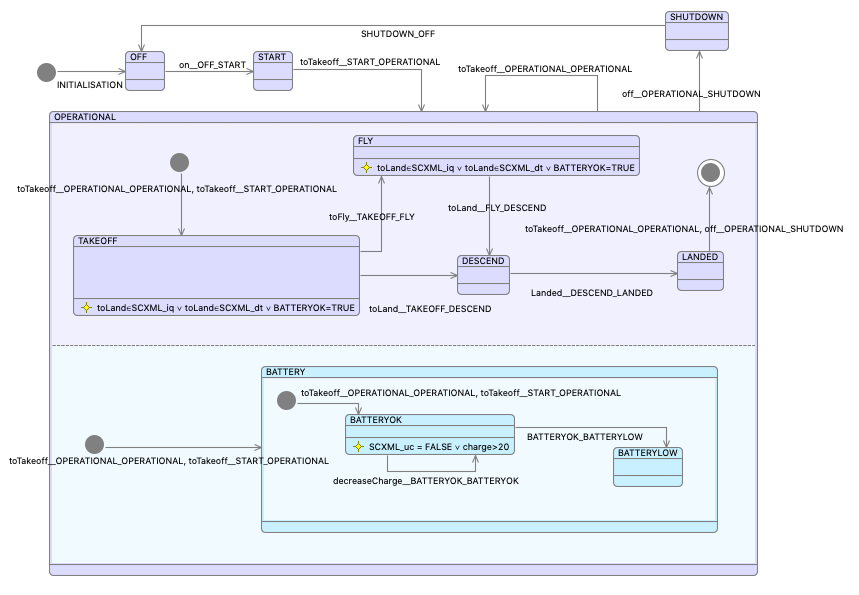
\includegraphics[width=0.90\textwidth, trim=0 40 0 0]{figures/drone2UMLB.png}
	\caption{Generated UML-B State-machine for drone refinement level 2. }
	\label{fig:drone2UMLB}
%	\vspace{-.4cm}
\end{figure} 

%%% Local Variables:
%%% mode: latex
%%% TeX-master: "../main"
%%% End:
% % !TEX root = ../main.tex

\section{State-chart Refinement}
\label{sec:scref}

Our system includes three refinement rules.

\begin{enumerate}
\item Guard conditions on a transition can be strengthened; 
this can done by adding textual guards to the transition, or
changing the source of the transition to a nested state.
\item Transitions can have additional actions, provided they do not
  modify variables appearing in the abstraction; this can be 
  accomplished by adding textual action to the transition 
  or by changing the target to nested state.
\item A state-chart can be embedded within a state of another
  state-chart -- sometimes called hierarchical composition or
  hierarchical refinement.
\end{enumerate}

Via the translation explained in Section~\ref{sec:translation}, these rules
rely on the usual \EventB proof obligations to ensure that they do
indeed yield refinements in the \EventB semantics.

If an \EventB model |B| can be shown (via the construction rules of
the \EventB language as well as the proof obligations) to refine
another \EventB model |A|, then we know that every behavior of |B| is
also a behavior of |A|. This definition yields a useful principle of
preservation of safety -- if we can show that a bad thing never
happens in |A|, then we can add detail via refinements in |B|, knowing
that the bad thing will continue to never happen in |B|. That is,
\EventB refinements preserve safety properties in the sense
of~\cite{lamport1977proving}. This makes refinement a useful technique
in developing safety-critical systems: one can analyze a simpler
abstract model for critical safety properties and then add detail to
the model via refinements, secure in the knowledge that the safety
properties will be preserved.

\EventB refinements have also been shown to preserve some liveness
properties, under certain conditions~\cite{hoang2016ltl}.

Although the autonomous drone example in this paper is based on the
example described in~\cite{Syriani_2019}, the definition of refinement
used in that work is quite different from our own. This forces some
differences in our refinement rules and consequently the way the
example is developed. For example, the transition triggered by |toLand| 
(see ~\ref{fig:drone4} transition from |TAKEOFF| to |DESCEND|) 
adds new behaviour.
In~\cite{Syriani_2019} ``refinement'' is a
transformation of the model which preserves reachability of a state
with respect to sequences of inputs. This guarantees that a refinement
in their system will include all the behaviors of the abstraction,
while possibly adding others. While this notion of refinement seems
useful in certain contexts, unlike refinement in \EventB it does not
guarantee preservation of safety properties. Therefore it should be
considered less suited to development of safety-critical systems.


% !TEX root = ../main.tex


\section{Validation}
\label{sec:validation}

One of the attractions of `run to completion' style modelling languages such as \SCXML is their execution semantics which provides a method for animating models to validate their behaviour.
Our approach to \SCXML refinement retains a single \SCXML final model which can be animated using the existing \SCXML animation tools.
However, we would like to validate the developing \UMLB model at intermediate refinement levels.

In previous work~\cite{snook20JSA} we have developed a scenario-based approach to formal modelling using abstract scenarios to validate abstract models.
The method is supported by a `Scenario Checker' tool, based on the \PROB model checker, that allows scenarios to be recorded and then replayed to check that important state has not changed since the original run of the scenario.
The Scenario Checker supports the concept of a controller executing a process in response to changes in the environment which is similar to the run to completion concept addressed in our work here.
Events may be annotated as \emph{internal} to indicate that they should be fired automatically if enabled until none are enabled. 
Internal events may also be prioritised to give a simple representation of process order in the controller (even if it is left non-deterministic in the model).
The user only has to select external events that trigger the controllers responses.
Since our \SCXML derived models already contain an implementation of run to completion the support provided by the Scenario Checker is sufficient to validate this behaviour.
If desired, internal variables that represent the controllers processing (e.g. the \SCXML statechart states) can be annotated as \emph{private} so that only controller output is checked during replay.
To help visualise the state of the model, the generated \UMLB state-machine is animated during the scenario validation.

In Figure~\ref{fig:scenarioChecker} we show a previously recorded scenario being played back on the drone model.
The main (top-left) editing view shows the state-machine being animated; the model is currently in the fly state.
The bottom left view is the scenario checker control panel.
The top button shows that a pre-recorded scenario is being played back and beside it the enabled external operations are greyed out since manual selection is disabled during playback.
The main button to be used is the \emph{Big Step} button which fires the next step of the scenario.
The bottom-right view shows the history, listing the operations that have already been played.
This is the same as the \PROB history view (top-right), but organises operations into big step runs (an external followed by a sequence of internal operations.
The bottom-middle view shows the state of the main variables and compares to the state when the scenario was recorded.
In the example, a discrepancy has been detected since non-determinism in the raised triggers allowed |DESCEND| to be reached when the scenario was recorded, but the playback has chosen to enter |FLY| instead.


\begin{figure}[!h]
	\centering
	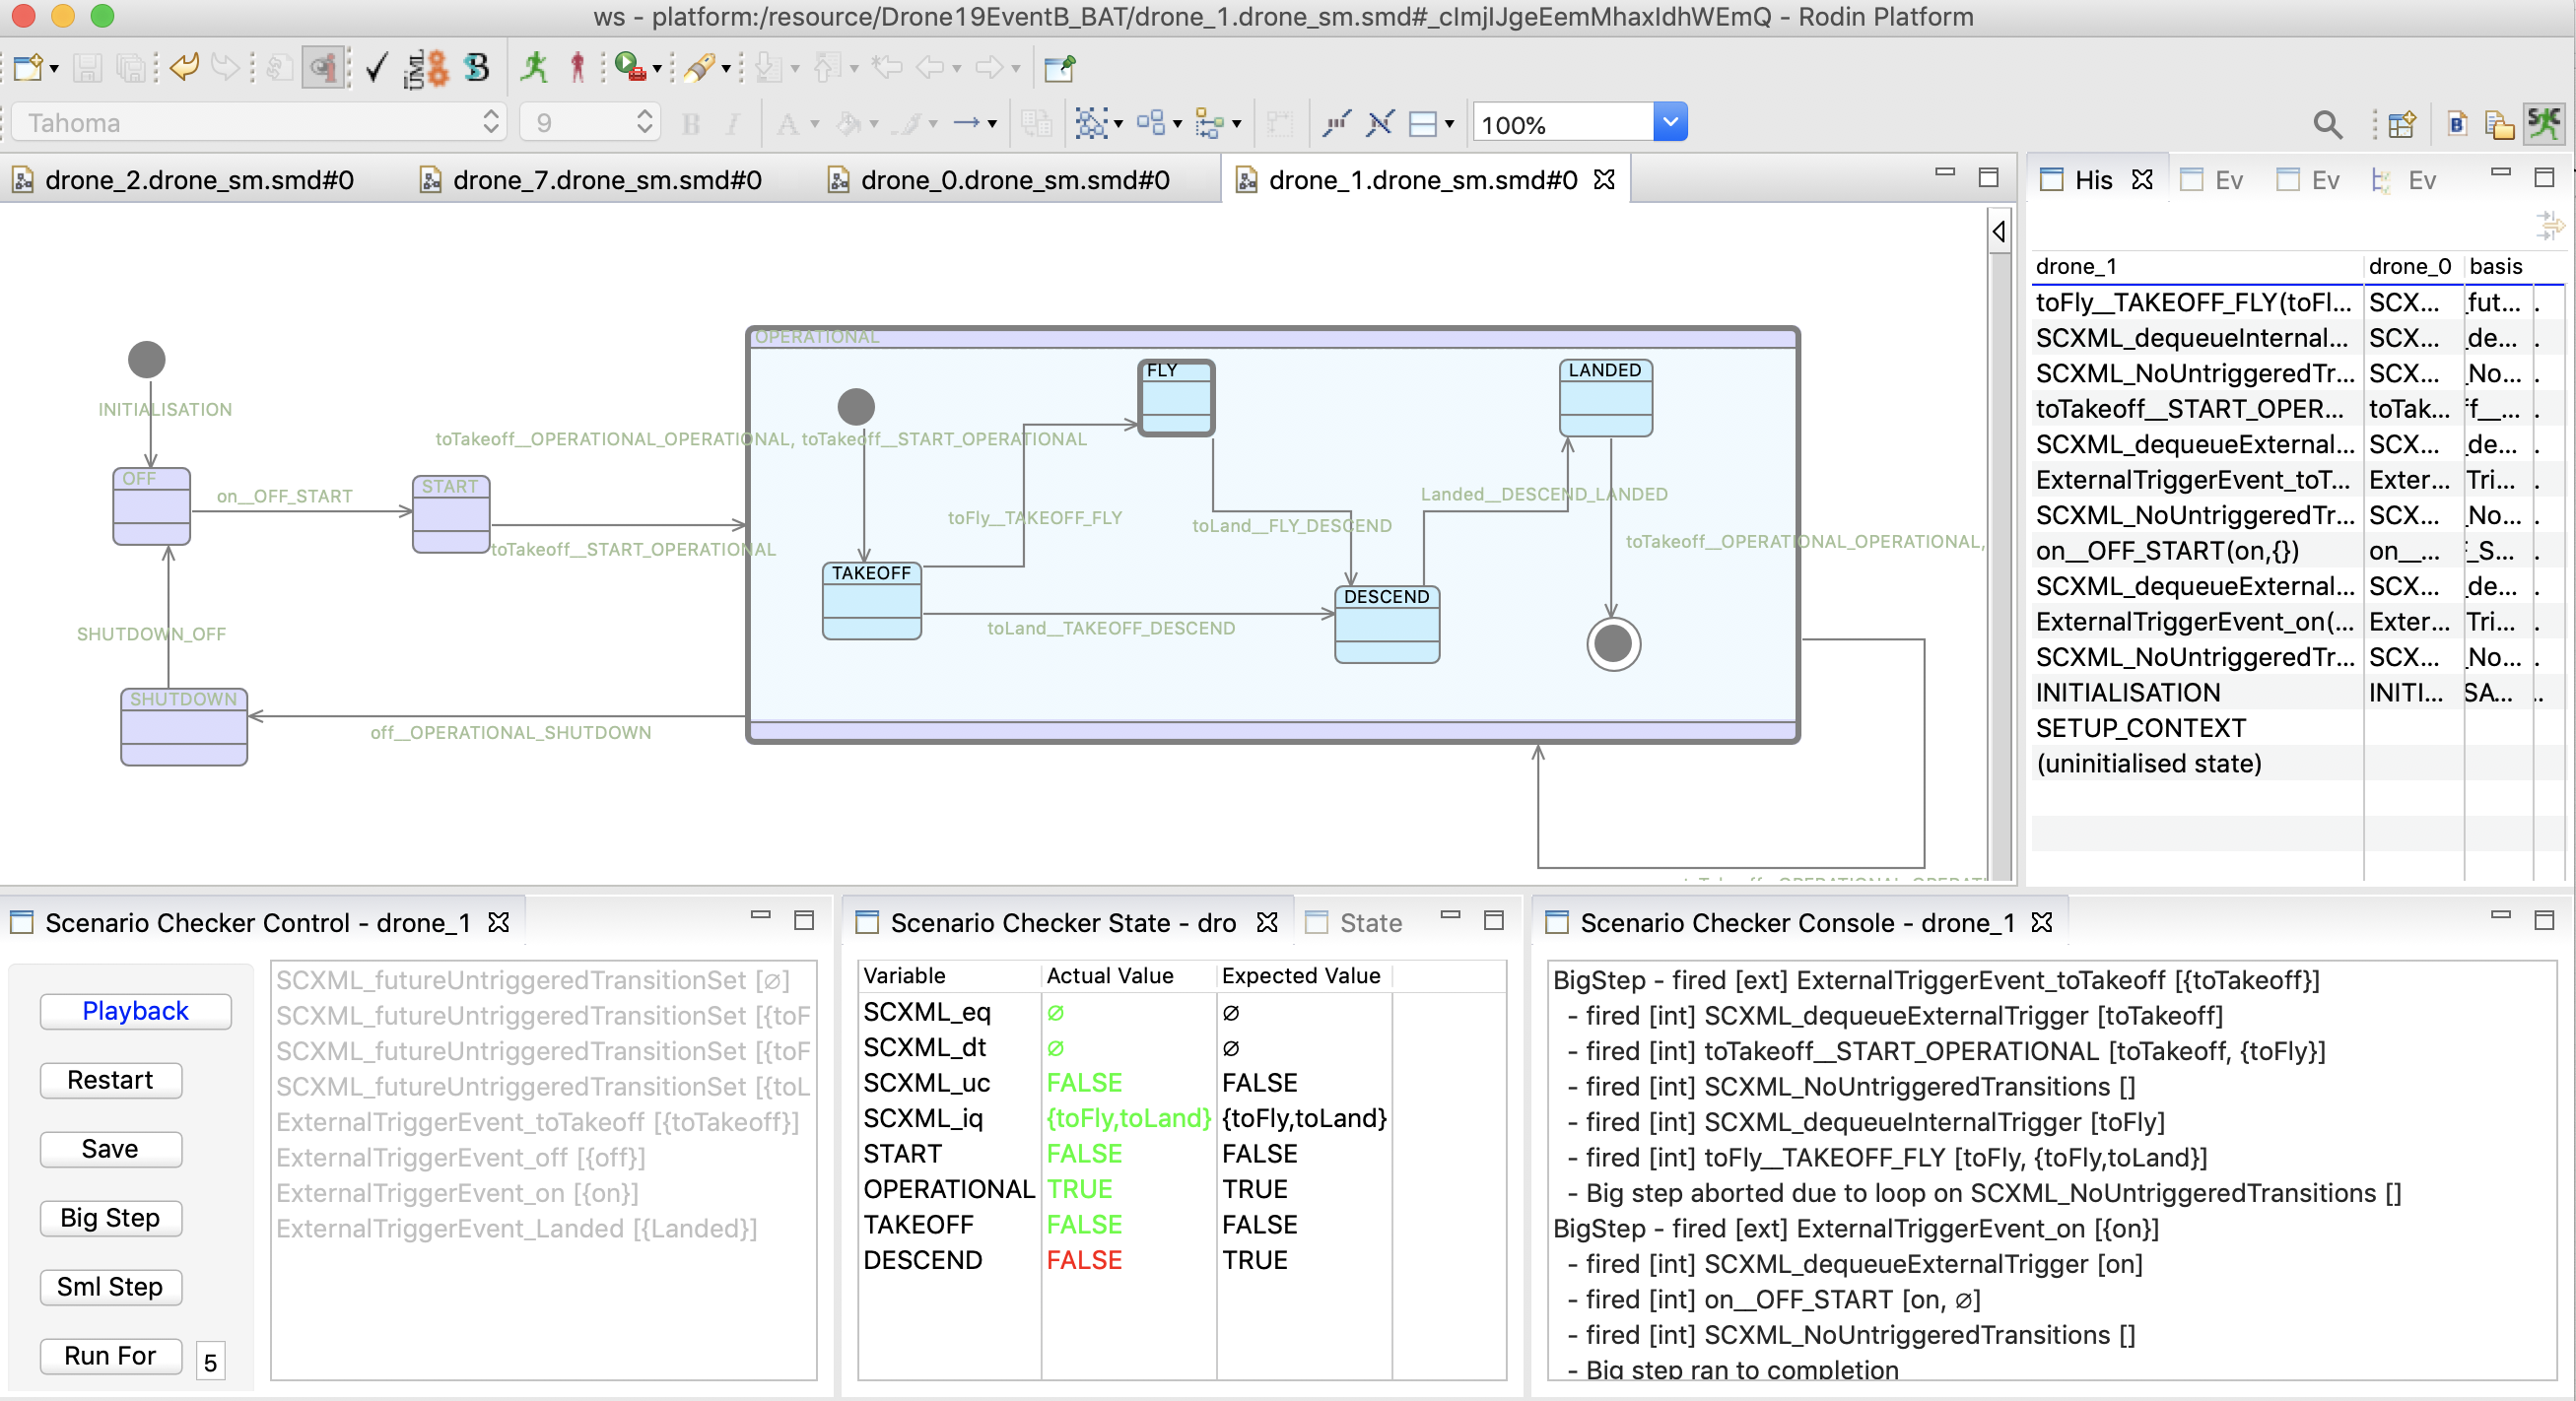
\includegraphics[width=0.90\textwidth, trim=30 50 60 0]{figures/scenarioChecker.png}
	\caption{Using Scenario Checker to validate behaviour}
	\label{fig:scenarioChecker}
\end{figure}

While the scenario checker allows us to animate the expected run to completion behaviour, recall that, unless the transitions have all been finalised (i.e. no further refinement is permitted),  other behaviours are possible due to the non-deterministic completion incorporated in case transition guards are later strengthened. 
The scenario checker allows the run to completion (i.e. internal events) to be overridden in order to explore these behaviours at an abstract level.
 

%%% Local Variables:
%%% mode: latex
%%% TeX-master: "../main"
%%% End:

% !TEX root = ../main.tex


\section{Verification of Safety Properties}
\label{sec:verificationSafety}

\todo{Merge the 2 verification section into one. And just the general form of the properties that can discharge automatically}
In a state-chart model we naturally wish to verify properties |P|, about other parallel statechart regions and auxiliary data, that are expected to hold true in a particular state |S|.
Hence, all of the safety properties that we consider are of the form: |S=TRUE ⇒ P|, where the antecedent is implicit from the containment of |P| within |S|.
%
%There are two kinds of properties that we might want to verify in an \SCXML state-chart;
%1) properties concerning the values of auxiliary data maintained by the system and 
%2) constraints about the state of another parallel state-chart region.

\SCXML models represent components that respond to received triggers and are not perfectly synchronised with changes in the monitored properties. 
Hence, |P| may be temporarily violated until the system responds by leaving the state |S| in which the property is expected to hold.
To cater for this we express |P| in a modified form |P'| that allows time for the response to take place.
There are two forms of reaction that can be used to exit |S|; 
a) an untriggered transition, or 
b) a transition that is triggered by an internally raised trigger.
For a), the modified property |P'| becomes |P ∨| \emph{untriggered transitions are not complete}, 
and for b) |P'| becomes |P ∨| \emph{trigger} |t| \emph{is in the internal queue or dequeued}
(where |t| is the internal trigger raised when the violation of |P| is detected).

%Not sure the following is true so removed it..
%For properties about the value of auxiliary data, untriggered transitions appear to be more suited because, in this case, there is unlikely to be a natural place to raise an internal trigger when the appropriate conditions arise.
%For properties about the state of a parallel region either reaction could be used depending on whether the system detects the violation in the state that contains P of the state that P refers to.

\todo{Insert a general form of the sort of properties we can verify and discuss} 
% In this section we illustrate a typical example of the type of properties that we imagine could be verified in a reactive \SCXML system.
% All of the proof obligations are automatically discharged for our example.
% Since our models are strictly structured and proof obligations will always have this common form, we are optimistic that proofs will always discharge automatically.
% We model the safety property features at an early level of refinement where the models are relatively simple, so that the validity of verification conditions is clear. 
% Detail is then added in later refinements which are proven (automatically) to preserve the previously verified safety properties.
% In our example, some auxiliary data is monitored by one state-chart region and while a parallel region refers to the state of the monitoring region. 
% Hence the reaction consists of an un-triggered transition in the monitoring region which sends an internal trigger to the other region when it leaves the desired monitor state.

% For our drone model, the safety property that we wish to verify is that the control system does not continue to take off or fly if the battery charge drops below a certain threshold (say 21\%). 
% By refinement level 1 we have developed the drone's state to the point where we distinguish the |TAKEOFF| and |FLY| states (Figure~\ref{fig:drone1}).
% In refinement level 2 we therefore introduce the battery charge monitoring function along with the associated safety properties.
% A parallel state-chart region, with sub-states |BATTERYOK| and |BATTERYLOW|, is added to the state |OPERATIONAL| (Figure~\ref{fig:drone4}).
% The |BATTERYOK| sub-state is used in the safety invariant of the |TAKEOFF| and |FLY| states.
% Thus we split the verification into two parts: a \emph{type b} proof to show that the system reacts to the battery charge decreasing below 21\% (an external event) by leaving the  |BATTERYOK| sub-state, and a \emph{type a} proof to show that when the system leaves the |BATTERYOK| state it subsequently (within the run to completion) leaves the |FLY| or |TAKEOFF| states. 
% Both parts are described in more detail as follows.

% \paragraph{System Reacts to the Low Battery Charge}
% An external trigger indicates that the battery charge has dropped by 10\% and this is used by a self transition to decrement the controllers data value for charge.
% The |BATTERYOK| state is supposed to indicate that the battery charge is ok ($>$20\%) and to ensure that it does, we add a state invariant to this effect (charge$>$20).
% When charge decreases to 20 (or less), an untriggered transition immediately reacts by switching to the |BATTERYLOW| state.
% To ensure that this reaction is not bypassed by the non-determinism that we incorporated to allow for future refinement, we flag it as finalised at refinement level 2.
% Finalisation means that we cannot strengthen its guards in future refinements as is normally permitted, since its reaction is needed to ensure the invariant is preserved.
% After translation to 
% %\UMLB and then \EVENTB
% \EVENTB via \UMLB
% the invariant in state |BATTERYOK| is 
% %|uc = FALSE ∨ charge>20| and after translation to \EVENTB, 
% \begin{center}
%  |(BATTERYOK = TRUE) ⇒ (uc = FALSE ∨ charge>20)|~.
% \end{center}
% The only events that can break this invariant are ones that make the antecedent become true or the consequent become false and we deal with these as follows:
% The transitions that enter state |OPERATIONAL| and initialise the |BATTERY| region by entering |BATTERYOK| (hence making the antecedent become true) contain the guard that |charge>50| (since we do not allow the drone to take off unless the battery is well charged) and hence the invariant is satisfied.
% The self transition that decreases charge (and hence could potentially falsify the consequent) is guarded by |uc = FALSE| since it is a triggered transition, and hence the disjunction in the consequent ensures it remains true.
% The completion event |NoUntriggeredTransitions| of the basis machine resets |uc = TRUE| to indicate completion of the cycle and hence could potentially break the invariant. 
% However, finalising the transition |BATTERYOK_BATTERYLOW| (that leaves |BATTERYOK| when |charge>20| becomes false) means that  the negation of its guard is added to the completion event by the translation.
% Since this transition fires when |BATTERYOK = TRUE| (i.e. its source state) and |charge≤20| the completion event is guarded by |¬(BATTERYOK= TRUE ∧ charge≤20)| which means that it does not fire when it could break the invariant (i.e. forcing the untriggered reaction to fire first).

% \paragraph{System Subsequently Leaves the FLY or TAKEOFF States}
% The safety property of the |TAKEOFF| and |FLY| states can now be simply stated as |BATTERYOK = TRUE|. 
% However, since this relies on a particular internal trigger (|toLand|) to make the appropriate reaction, we also need to specify that trigger as an attribute of the invariant in the \SCXML model.
% After translation to \EVENTB via \UMLB the invariant in state |TAKEOFF| becomes 
% \begin{center}
%  |(TAKEOFF = TRUE) ⇒ (toLand∈iQ ∨ toLand∈dt ∨ BATTERYOK=TRUE)|.
% \end{center}
% The invariant for the |FLY| state is similar with a corresponding antecedent.
% The transitions that enter |TAKEOFF| (which make the antecedent true) simultaneously enter |BATTERYOK| ensure the consequent is true.
% The only transition that enters |FLY| (which makes the antecedent of the |FLY| invariant true) comes from the |TAKEOFF| state and hence the consequent is already true.
% The transition that leaves |BATTERYOK| (making the last disjunct of the consequent false) raises the |toLand| trigger making the first disjunct true.
% Some transitions leave the superstates of |BATTERYOK| but these either simultaneously leave |OPERATIONAL| (the superstate of |TAKEOFF| and |FLY|), or re-enter |BATTERYOK|.
% The basis contains an event to dequeue the internal triggers which preserves the overall consequent because establishes the second conjunct as it falsifies the first (i.e. it removes |toLand| from the |iQ| but simultaneously adds it to |dt|).
% The only events that falsify the second conjunct are the transitions triggered by |toLand| which leave the |TAKEOFF| or |FLY| states making the antecedent false.

% Hence, invariant properties that follow these suggested patterns are always automatically proven due to simple logic about the changes in state.

%%% Local Variables:
%%% mode: latex
%%% TeX-master: "../main"
%%% End:

% !TEX root = ../main.tex
\section{Verification of Control Responses}
\label{sec:verificationResponses}

A model that has been proven to satisfy some safety (e.g., invariant)
properties, may still not behave in a useful way.  Therefore, as well
as verifying invariant properties, we would like to verify the
system's liveness (e.g., responsive) properties. That is, we want to
ensure that the controller responds to external triggers and makes
appropriate modifications to the system variables.  These kind of
liveness properties are difficult to prove via invariant preservation
since they are temporal properties.  In this section, we present our
approach to verify the responsive properties of the system.

We first start with some generic properties of our generated \EventB
model and the fairness assumption about the executions of the events.
We then discuss the proof for termination of responses for external
triggers in Section~\ref{sec:contr-rema-resp} and correctness of the
responses for external triggers in Section~\ref{sec:corr-resp-extern}.

\paragraph{Event Categories.} In our \EventB model, the events can
be separated into the following categories.
\begin{itemize}
\item \emph{External events}: These events raise external triggers.
  
\item \emph{System events}: Events other than external events are
  called system events. They are the events by which the system
  responds to the external triggers (by creating 
  different runs or simulation paths).
  These events can be seen in Figure~\ref{fig:basis} and are further
  categorised as follow.
  \begin{itemize}
  \item \emph{Future system events}: These events might raise internal
    triggers, i.e., |futureTriggeredTransitionSet|, and
    |futureUntriggeredTransitionSet|.  The purpose of these events is
    to enable future introduction of more system details via
    refinement.
    
  \item \emph{The dequeue external trigger event} (i.e.,
    |dequeueExternalTriggered|): These events dequeue the
    external trigger queue and will start a run.

  \item \emph{Internal system events}: These events belong to the
    internal behavior of the system to accommodate the runs for external
    triggers.  These events can be seen in different groups as in
    Figure~\ref{fig:basis}.
    \begin{itemize}
    \item \emph{The dequeue internal trigger event} (i.e.,
      |dequeueInternalTriggered|): These events dequeue the
      internal triggers queue and will start a run.
    
    \item \emph{Triggered events}: The events corresponding to the
     event fired by (external or internal) triggers.

    \item \emph{The discard trigger event} (i.e.,
      |noTriggeredTransitionsEnabled|):  This event will move the system
      from the |FIRING TRIGGERED| state to the |FIRING UNTRIGGERED| state 
      in the case where no triggered transition events are enabled.
    
    \item \emph{Untriggered events}:  These are all the untriggered 
    events in the systems.

    \item \emph{The completion event} (i.e.,
      |noUntriggeredTransitionsEnabled|): This event will move the
      system from |FIRING UNTRIGGERED| state to the |READY TO DE-QUEUE|
      state in the case where no untriggered transition events are
      enabled.
    \end{itemize}
  \end{itemize}
\end{itemize}
Events from different categories have different roles in our reasoning
about responsive properties.

We now present a theorem and a corollary related to (relative)
deadlock-freeness properties for a different set of events.
\begin{theorem}[Internal System Events are Relative Deadlock-Free]
  \label{thm:Internal-DLF}
  Under the condition that %
  |iQ /= {} !or uc = FALSE !or dt /= {}|, %
  the internal system events are deadlock-free, i.e., there must be
  one internal system event enabled.
\end{theorem}
\begin{proof}
  This is based on the generation of our \EventB model (according to
  the basis structure as seen in Figure~\ref{fig:basis}).  In
  particular, we consider the different cases corresponding to the
  different ``states'', i.e., |READY TO DE-QUEUE|, |FIRING TRIGGERED|,
  and |FIRING UNTRIGGERED|.
  \begin{itemize}
  \item When the system is in the |READY TO DE-QUEUE| state, we know
    that %
    |uc = TRUE & dt = {}|.  %
    According to our assumption, we then have |iQ /= {}|, hence
    |dequeueInternalTriggered| event is enabled.
    
  \item When the system is in the |FIRING TRIGGERED| state,
    either one of the triggered events is enabled or the
    |noTriggeredTransitionsEnabled| event is enabled.
    
  \item Similarly, when the system is in the |FIRING UNTRIGGERED|
    state, either one of the untriggered events is enabled or the
    |noUntriggeredTransitionsEnabled| event is enabled.  
  \end{itemize}
  \qed
\end{proof}
    
\begin{corollary}[System Events are Relative Deadlock-Free]
  Under the condition that %
  |eQ /= {} !or iQ /= {} !or uc = FALSE !or dt /= {}|, %
  the system events are deadlock-free, i.e., there must be
  one system event enabled.
\end{corollary}
\begin{proof}
  This is based on the generation of our \EventB model (according to
  the basis structure as seen in Figure~\ref{fig:basis}) and
  Theorem~\ref{thm:Internal-DLF}.
  \begin{itemize}
  \item In the case where |iQ /= {} !or uc = FALSE !or dt /= {}|,
    according to Theorem~\ref{thm:Internal-DLF}, one of the internal
    events is enabled.
    
  \item Otherwise, i.e., |iQ = {} & uc = TRUE & dt = {}|, according to
    our assumption, |eQ /= {}|. In this case, the
    |dequeueExternalTriggered| event is enabled.
  \end{itemize}
  \qed
\end{proof}

In order to reason about any liveness properties for an event system,
we have to make assumptions about how often events will be fired.
Here, we assume that all the system events are strongly fair.
\begin{assumption}[Fair System Events]
  \label{asm:SF}
  % \SonChange{%
  %   We assume that all system events are strongly fair, i.e., if a
  %   system event is enabled infinitely often, eventually, it will be
  %   eventually fired.%
  % }{%
  \hl{%
    We assume that all internal system event \mbox{\EventBInline{e}}
    are strongly fair, i.e., \mbox{\EventBInline{SF(e)}}; and the
    dequeue external trigger event is weakly fair,
    i.e., \mbox{\EventBInline{WF(dequeueExternalTriggered)}}.%
  }
\end{assumption}
This assumption will ensure that the system will response no matter
how often the external triggers are raised by the external events.

\subsection{Termination of Responses for External Triggers}
\label{sec:contr-rema-resp}

We first define the notion of event convergence and event
anticipation.
\begin{definition}[Event Convergence]
  \label{def:conv}
  A set of events is said to be convergent if they all \emph{decrease}
  a variant according to some well-founded order.
\end{definition}

\begin{definition}[Event Anticipation]
  \label{def:anticipated}
  Given a set of convergent events with respect to a variant,
  another set of events is anticipated with respect to the
  same variant if they \emph{do not increase} the variant.
\end{definition}
\hl{%
  Note that the anticipated events augment the set of convergent
  events and respect the variant used to prove the
  convergence property.% 
}

We start first by stating the main theorem about termination of
responses for external triggers: it is always the case that the system
will comeback to the |READY TO DE-QUEUE| state and |iQ = {}|, i.e.,
the system is ready to dequeue an external trigger (if any).  This is
stated as the following theorem.
\begin{theorem}[Termination of Internal System Events]
  \label{thm:finite-internal-events}
  Given that the internal events are convergent and the external
  events are anticipated, the system's internal queue is always
  eventually empty and the system transitions to the \emph{Ready to
    De-queue} state, i.e.,
  \begin{center}
    |GF(iQ = {} & uc = TRUE & dt = {})|~.
  \end{center}
\end{theorem}
\begin{proof}
  Assuming that the properties is not satisfied, i.e., eventually,
  it is always the case that %
  |iQ /= {} !or  uc = FALSE !or dt /=  {}|.  %
  This can be formalised as follows.
  \begin{center}
    |FG(iQ /= {} !or uc = FALSE !or dt /= {})|~.    
  \end{center}
  Observe that in the states satisfying this condition, the
  |dequeueExternalTriggered| event is disabled.  Furthermore,
  according to Theorem~\ref{thm:Internal-DLF}, the internal events
  will always be deadlock-free, and as a result, at least one of the
  internal event is enabled infinitely often\hl{, hence under the
    Assumption~\mbox{\ref{asm:SF}}, this event occure infinitely
    often}. According to Definition~\ref{def:conv}, the variant will
  be decreased infinitely which violate the condition that the variant
  is defined on an well-founded order.  Here, the external events are
  anticipated to ensure that the variant does not increase, hence does
  not interfere with the convergence of the internal events.%
  \qed
\end{proof}
\hl{%
  Note that Theorem~\mbox{\ref{thm:finite-internal-events}} relies on
  convergence of internal events and anticipation of external events,
  which we will prove later.%
}

\begin{theorem}[Responsiveness to External Triggers]
  \label{thm:resp-ext-trg}
  If an external trigger is raised, then eventually, it will be dequeued.
  \begin{center}
    |G([externalTrigger.t] => F([dequeueExternalTriggered.t]))|~,
  \end{center}
  where we use |externalTrigger.t|
  (resp. |[dequeueExternalTriggered.t]|) to denote the occurrence of
  |externalTrigger| (resp. |dequeueExternalTriggered|) with parameter |t|.
\end{theorem}
\begin{proof}
  Assuming that |[externalTrigger.t]| hence |t !: content(eQ)|, i.e.,
  |eQ /= {}|.  According to Theorem~\ref{thm:finite-internal-events},
  we have that |dequeueExternalTriggered| is enabled infinitely often.
  Since |dequeueExternalTriggered| is weakly-fair
  (Assumption~\ref{asm:SF}), it is taken infinitely. We have two
  cases.
  \begin{itemize}
  \item If |t = head(eQ)|, it means we have
    |[dequeueExternalTriggered.t]|
    
  \item If |t /= head(eQ)|, an occurrence of |dequeueExternalTriggered|
    will move |t| closer to be the head of the external queue |eQ| and
    eventually it will become the head of the queue and subsequently
    be processed eventually.
  \end{itemize}
  \qed
\end{proof}

\subsubsection{Proof of Convergence and Anticipation}
\label{sec:proof-convergence}
The responsiveness to external triggers presented in
Theorem~\ref{thm:resp-ext-trg} relies on
Theorem~\ref{thm:finite-internal-events}, which in turn relies on the
proof of convergence for internal system events and anticipation for
external events.  These proof will need to be done for each individual
SCXML state-chart as they do not hold a priori.  We present a
systematic approach to reason about the proof of convergence and
anticipation relying on lexicographic order as follow.

A variant in \EventB can be a natural number (bounded bellow by |0|)
or a finite set (bounded below by the empty set |{}|).  Moreover, for
a set of events, the variants $V_1, V_2, ...$ are combined into a
lexicographic variant, i.e., $(V_1, V_2, ...)$ with $V_1$ has a higher
priority than $V_2$, etc. An event is said to decrease this
lexicographic variant if it either decreases $V_1$ or if it keeps
$V_1$ the same and decreases $V_2$, so on and so forth.  Lexicographic
variants are supported in the latest Rodin (version 3.5).

Our generic approach to construct a lexicographic variant is according
to the following order and the rule for each variant.
\begin{enumerate}
\item $V_{externalTrigger}$ = |dt /\ ExternalTrigger|.  This variant
  is used to prove the convergence for any externally triggered events
  (i.e., triggered event by some external trigger). These event remove
  the external trigger from |dt| hence ``decrease'' |dt| to the empty
  set.

\item \label{variant:sm} Variants based on the state machine to prove
  the convergence of internally triggered events and untriggered
  events.  This depends on the SCXML diagram and we will illustrate
  this on the example later.
  
\item $V_{dequeueInternalTriggered}$ = |length(iQ)|.  This variant is
  used to prove the convergence of the |dequeueInternalTriggered| event.
  Since this event remove the head of the |iQ|, it decreases the
  length of the |iQ| trivially.  While other events might increase
  |iQ|, by raising new internal triggers. However, these events should
  have been proved to converge using higher-priority variants.
  
\item $V_{noTriggeredTransitionsEnabled}$ = |dt|.  This variant is used to
  prove the convergence of the |noTriggeredTransitionsEnabled| event.
  The event discard the trigger in |dt| hence ``decrease'' |dt| to the
  empty set.
  
\item $V_{noUntriggeredTranstitionsEnabled}$ = |{uc, TRUE}|.  This variant is
  used to prove the convergence of the
  |noUntriggeredTransitionsEnabled| event.  The event changes |uc|
  flag from |FALSE| to |TRUE|, hence ``decrease'' the variant from
  |{FALSE, TRUE}| to |{TRUE}|.
\end{enumerate}
\hl{%
  Note that except for the variant related to the internally triggered
  events and untriggered events, i.e., \mbox{(\ref{variant:sm})}, all
  other variants, i.e., $V_{externalTrigger}$,
  $V_{dequeueInternalTriggered}$, $V_{noTriggeredTransitionsEnabled}$,
  and $V_{noUntriggeredTranstitionsEnabled}$ are generic according to
  the underlying run-to-completion semantics.%
}

The external events are anticipated according to the above variants
trivially since they only modify the external queue |eQ|.  Note that
we do not attempt to prove the convergence of any future events
here. Instead, we assume that these future events will be proved to be
convergent later.

% Order of the variants
We now discuss the specific variants for the Drone example based on
the actual state-chart as showed in Figure~\ref{fig:drone4}.  The
variants are for the internally triggered events and untriggered
events. The lexicographic order of the variant use to prove the
convergence of the events depending (1) on the \emph{nested structure}
of the state-chart and (2) on the \emph{order of the transitions} with
the same state-chart.  For example, the variant for proving the
convergence for the transition from |SHUTDOWN| to |OFF| will have a
higher priority than the one for the transition from |TAKEOFF| to
|FLY|, and this variant subsequently has higher priority than the one
for the transition from |CLIMB| to |HOVER|.  Furthermore, the variant
for proving the convergence for the transition from |TAKEOFF| to |FLY|
has higher priority than the one for the transition from |FLY| to
|DESCEND|.

% Shape of the variants
The translation of SCXML state-chart into UML-B/\EventB represents each
state by a Boolean variable, |TRUE| if the system in that state and
|FALSE| otherwise. As a result, the variant for proving the convergence
of an event going out of a state |S| can be |{S, FALSE}|: the
transition ``decreases'' the value of the variant from |{TRUE, FALSE}|
to |FALSE|.

Based on the above analysis, the variants that we used for proving the
convergence of the internally triggered events and untriggered events
in the Drone example are.
\begin{itemize}
\item |{SHUTDOWN, FALSE}|

\item |{TAKEOFF, FALSE}|

\item |{FLY, FALSE}|

\item |{BATTERYOK, FALSE}|

\item |{CLIMB, FALSE}|

\item |{CLIMB2, FALSE}|
\end{itemize}

This variant proof are available in the Rodin archive at
\url{https://tinyurl.com/ISSE-Drone}.


\subsection{Correct Responses to External Triggers}
\label{sec:corr-resp-extern}
In the previous section, we illustrate the reasoning about the
responsiveness of the system to external triggers.  However, we also
need to prove that the response to the external triggers is correct.
In our conference paper~\cite{detect2020}, we illustrate the use of
ProB model checker to reason about such a property.  Here, we show how
we can prove such a property.

%\SonInlineComment{We should probably move this to the discussion}
% While \EventB refinements have also been shown to preserve some liveness properties under certain conditions~\cite{hoang2016ltl}, there are not yet efficient supporting tools for the technique.%
% \SonComment{We probably need to move this to related work}
% Instead, we can express the property in \LTL  and use the \PROB\footnote{ProB is an animator, constraint solver and model checker for the B-Method. https://www3.hhu.de/stups/prob} model checker to verify it.

Once again, we assume that the system events are strongly fair as in
Assumption~\ref{asm:SF}.  In general, our correct-response properties
will have the following form:
\begin{center}
  |G([external_trigger_event] => F{predicate})|~,
\end{center}
where the predicate concerns variables |v| that the system maintains,
and may refer to old values |old(v)| that existed when the external
trigger occurred.  The translator generates a separate `branch'
refinement for each \LTL property to be verified.  In this special
refinement, history variables are added to record the value at the
state when the external trigger occurs, of any variables that are
referenced as `old' values.

We illustrate the method with an example of a temporal property that
we expect to hold in the drone \SCXML system.  The liveness property
that we wish to verify is that, after an external trigger event
|decreaseCharge|, the battery charge value should decrease in value, i.e.,
\begin{center}
  |G ([ExternalTriggerEvent_decreaseCharge] => F {charge < old(charge)})|~.
\end{center}
As discussed in~\cite{detect2020}, this above property is too strong
and does not hold for the SCXML drone model.  We have to weaken the
property to state that the expected behaviour is only achieved if the
external trigger is raised at the right time specified as %
|{BATTERYOK=TRUE & charge>20}|, %
and there are no external conflict triggers, here |off|, in processing
or that has been raised, i.e., %
|off /: dt \/ content{eQ}|.  %
The property can be formalised as follows

\begin{center}
  |G([ExternalTriggerEvent_decreaseCharge] & |\\
  |{BATTERYOK=TRUE & charge>20 & off/:dt & off /: content(eQ)}|\\
  |=> F {charge < old(charge)})|~.
\end{center}
In order to prove the above property, we first recall the definition
of \textbf{unless}
property~\cite{DBLP:books/daglib/0067338,hudon16:_unit_b_method}.
\begin{definition}[Unless Properties]
An \emph{unless property} of the
following form
\begin{center}
  |P| \textbf{unless} |Q|
\end{center}
means that if |P| holds then it will hold continuously unless |Q| hold.
\end{definition}
We restate the \emph{Unless rule} (Theorem 1
in~\cite{hudon16:_unit_b_method}) here.
\begin{theorem}{Unless rule}:
  \label{thm:unless-rule}
  An event system satisfies the unless property |P| \textbf{unless}
  |Q|, if for every event, if it starts in a state satisfying %
  |P & !not Q|, %
  it will reach a state satisfying %
  |P !or Q|.  %
\end{theorem}

Coming back to our example, we first prove that the \EventB model
satisfies the following important \textbf{unless} property.
\begin{theorem}
  \label{thm:unless}
  The drone system satisfies the following \textbf{unless}
  property.

  \begin{center}
    |BATTERYOK = TRUE & charge > 20 & decreaseCharge !: content(eQ) & off /: dt &|\\
    |(! i  !: dom(eQ) . eQ(i) = off => (#j !: dom(eQ) . eQ(j) = decreaseCharge & j < i))|\\
    \textbf{unless} \\
    |BATTERYOK = TRUE & charge > 20 & dt = {decreaseCharge}|\\
  \end{center}
\end{theorem}
\begin{proof}[Sketch]
 The proof relies on Theorem~\ref{thm:unless-rule}, i.e.,
 reasoning per event.  The encoding of the proof obligations are
 available from the Rodin archive. We informally explain why this
 property holds for different class of events below.
 \begin{itemize}
 \item \emph{External events}: The external events raise a new external
   trigger and append the new trigger to |eQ|. Given that
   |decreaseCharge| is already in |eQ|, even if the new trigger is
   |off|, this trigger cannot over take |decreaseCharge| in the queue,
   i.e., it is alway behind |decreaseCharge|. These external events
   therefore maintains the left-hand side of the \textbf{unless} property.
   
 \item \emph{Dequeue external trigger}: If the dequeued external
   trigger is |decreaseCharge|, we will have |dt = {decreaseCharge}|,
   hence we establish the right-hand side of the unless property.
   If it is not |decreaseCharge|, it also cannot be |off| (as any
   |off| trigger in |eQ| has to be behind a |decreaseCharge|
   trigger). As a result, the condition that |off| is behind
   |decreaseCharge| in the remaining queue is maintained and
   |off| cannot be in |dt| after the event execution.
   
 \item \emph{Internal system events}: For the internal systems events,
   we separate them into those that are outside the |BATTERY| state
   and those that are inside of the |BATTERY| state.
   \begin{itemize}
   \item For those that are outside the |BATTERY| state, they maintain
     the left handside of the unless property trivially (by leaving
     external queue unchanged and does not alter the relevant state,
     i.e., |BATTERY| or the |charge|).
     
   \item For the self-transition which is triggered by
     |decreaseCharge| inside the |BATTERY| state, the proof of the
     unless property is trivial, since we assume the negation of the
     right-hand side of the unless property, including that that
     |decreaseCharge| is not in |dt|. For the transition from
     |BATTERYOK| to |BATTERYLOW|, the proof of the unless property is
     also trivial, since we assume the left-hand side of the unless
     property, including that |charge > 20|.
   \end{itemize}
 \end{itemize}
 \qed
\end{proof}
Theorem~\ref{thm:unless} means that the system will continuously
satisfy the following conditions:
\begin{itemize}
\item in the |BATTERYOK| state~,
  
\item |charge| is more than |20|~,
  
\item |decreaseCharge| is in the external queue |eQ|~.
  
\item |off| is not in |dt|~.
  
\item if |off| is in the external queue |eQ| then it is behind a
  |decreaseCharge| trigger~.
\end{itemize}
\textbf{unless} it reaches a state satisfying the following conditions:
\begin{itemize}
\item in the |BATTERYOK| state~,
  
\item |charge| is more than |20|~,
  
\item |decreaseCharge| is in |dt|.
\end{itemize}

Coming back to the proof for our correct-response property and assume
that the system is at the right time and the
|[ExternalTriggerEvent_decreaseCharge]| event happens.  Notice that at
that particular moment, the left-hand side of the progress property in
Theorem~\ref{thm:unless} is also satisfied.  According to
Theorem~\ref{thm:resp-ext-trg}, eventually,
|[dequeueExternalTriggered.decreaseCharge]| is fired (and %
|dt = {decreaseCharge}|), %
i.e., |decreaseCharge| is dequeued from the |eQ| into |dt|. And at
that time, according to Theorem~\ref{thm:unless}, we also have
|BATTERYOK = TRUE| and |charge > 20|.  That ensures the triggered
transition event for |decreaseCharge| is enabled (and it is the only
internal event enabled) and will be eventually taken, hence decrease
the |charge|'s value accordingly.


% \begin{center}
%   |G([ExternalTriggerEvent_decreaseCharge] & {BATTERYOK=TRUE & charge>=10 &|
%     |off/:dt\/content(eQ)}|
%   |=> ({BATTERYOK=TRUE & charge>=10 & off /: dt & decreaseCharge :
%     content(eQ) & (! i . eQ(i) = off => (#j . eQ(j) = decreaseCharge &
%     j < i))} U {decreaseCharge =
%   head(eQ)}|
% \end{center}

% To specify a liveness property to be verified, a special \LTL element is added to the \SCXML model with attributes, property (a string of the above form)  and refinement (an integer indicating the refinement level at which the property should be verified).

% A text file is automatically generated containing the \LTL property to be checked. 
% In this generated version, an assumption of strong fairness is added for all other events in the model.
% Without this assumption, the system may never achieve the expected response to a trigger. 
% Therefore it corresponds to a requirement that the system can always make satisfactory progress and not become live locked.
%This assumption is stronger than necessary since some events will not affect the outcome, but is easier to generate and is sufficient for our verification aim. 
% For simplicity we omit this assumption from the remaining examples.
% \begin{center}
%   |SF[e1] & SF[e2]... => G([external_trigger _event] => F[predicate])|
% \end{center}
% This property can be added into the ProB model checker LTL formula text field.

% However, we could not verify this property.
% The counter example traces that \PROB provided gave us a better understanding of the reasons why. 
% The property as stated is too strong (i.e., not true) for our model; there are additional conditions that need to be considered and added as part of the antecedent.
% \begin{itemize}
% \item
% Our model represented the trigger queues abstractly as sets which meant that the |decreaseCharge| trigger may never be dequeued.
% The standalone version of \PROB allows strong fairness to be specified for particular parameter values but this does not work in the Rodin plug-in for \PROB. 
% In any case, a more accurate (concrete) representation of the queue fixes the problem and improves our model.
% \item 
% The charge is not always decreased in response to the |decreaseCharge| trigger.
% The controller only monitors battery charge while in the |BATTERYOK| state and discards the trigger in other states.
% Also, the controller stops decreasing charge when it approaches 0. 
% To cater for this we added a pre-condition %
% |BATTERYOK = TRUE ∧ charge > 20| %
% to the \LTL property.
% \item
% Even if this pre-condition is true when the trigger is raised, another trigger (e.g., |off|) may already be in the queue and take the controller out of |BATTERYOK| before the |decreaseCharge| trigger is dequeued.
% Again we strengthen the pre-condition |off ∉ dt ∪ eQ| of the \LTL expression to avoid this situation.
% \end{itemize}
% After making these changes the final form of the \LTL property, which \PROB was able to exhaustively check and confirm was as follows:
% \begin{center}
% 	|G([ExternalTriggerEvent_decreaseCharge] & {BATTERYOK=TRUE & charge>=10 &|
% 		|off/:SCXML_dt\/SCXML_eq} => F {charge < old(charge)})|~.
% \end{center}

%%% Local Variables:
%%% mode: latex
%%% TeX-master: "../main"
%%% End:

\section{Conclusion}

In conclusion ...

\vspace{6 pt}
\begin{scriptsize}
	
	\par
	\noindent
	All data supporting this study are openly available from the University of Southampton repository at
	https://doi.org/10.5258/SOTON/D1475\\

	\par
	\noindent
	\textbf{Acknowledgements} Sandia National Laboratories is a multimission laboratory managed and operated by National Technology \& Engineering Solutions of Sandia, LLC, a wholly owned subsidiary of Honeywell International Inc., for the U.S. Department of Energy’s National Nuclear Security Administration under contract DE-NA0003525.
	
\end{scriptsize}


\bibliographystyle{splncs04}
\bibliography{SCXMLREF}

\end{document}

%%% Local Variables: 
%%% mode: latex
%%% TeX-master: t
%%% End: 
